\documentclass[12pt]{report}
\usepackage[T1]{fontenc}
\usepackage[utf8]{inputenc}
\usepackage{caption}
\usepackage{adjustbox}
\usepackage{graphicx}
\usepackage{amsmath,amssymb,amsfonts}
\usepackage{txfonts}
\usepackage{listings}
\usepackage{float}
\usepackage{color}
\usepackage{xcolor}
\usepackage{enumitem}
\graphicspath{{images/}}
\renewcommand{\chaptername}{Rozdział}
\renewcommand{\contentsname}{Spis treści}
\renewcommand{\figurename}{Rysunek}
\renewcommand{\listfigurename}{Spis rysunków}
\renewcommand{\bibname}{Bibliografia}
\setlength{\textwidth}{14cm}
\setlength{\textheight}{20cm}
\newtheorem{definition}{Definicja}
\newtheorem{example}{Przykład}[chapter]
\lstdefinelanguage{JavaScript}{
  keywords={typeof, new, true, false, catch, function, return, null, catch, switch, var, if, in, while, do, else, case, break},
  keywordstyle=\color{blue}\bfseries,
  ndkeywords={class, export, boolean, throw, implements, import, this},
  ndkeywordstyle=\color{darkgray}\bfseries,
  identifierstyle=\color{black},
  sensitive=false,
  comment=[l]{//},
  morecomment=[s]{/*}{*/},
  commentstyle=\color{purple}\ttfamily,
  stringstyle=\color{red}\ttfamily,
  morestring=[b]',
  morestring=[b]"
}
\lstset{
   language=JavaScript,
   backgroundcolor=\color{lightgray},
   extendedchars=true,
   basicstyle=\footnotesize\ttfamily,
   showstringspaces=false,
   showspaces=false,
   numbers=left,
   numberstyle=\footnotesize,
   numbersep=9pt,
   tabsize=2,
   breaklines=true,
   showtabs=false,
   captionpos=b
}
\lstdefinelanguage{XML}
{
  morestring=[b]",
  morestring=[s]{>}{<},
  morecomment=[s]{<?}{?>},
  stringstyle=\color{black},
  identifierstyle=\color{blue},
  keywordstyle=\color{cyan},
  morekeywords={xmlns,version,type}% list your attributes here
}
\lstset{
  basicstyle=\ttfamily,
  columns=fullflexible,
  showstringspaces=false,
  commentstyle=\color{gray}\upshape
}
\colorlet{punct}{red!60!black}
\definecolor{background}{HTML}{EEEEEE}
\definecolor{lightgray}{rgb}{.9,.9,.9}
\definecolor{darkgray}{rgb}{.4,.4,.4}
\definecolor{purple}{rgb}{0.65, 0.12, 0.82}
\definecolor{delim}{RGB}{20,105,176}
\colorlet{numb}{magenta!60!black}
\lstdefinelanguage{json}{
    basicstyle=\normalfont\ttfamily,
    numbers=left,
    numberstyle=\scriptsize,
    stepnumber=1,
    numbersep=8pt,
    showstringspaces=false,
    breaklines=true,
    frame=lines,
    backgroundcolor=\color{background},
    literate=
     *{0}{{{\color{numb}0}}}{1}
      {1}{{{\color{numb}1}}}{1}
      {2}{{{\color{numb}2}}}{1}
      {3}{{{\color{numb}3}}}{1}
      {4}{{{\color{numb}4}}}{1}
      {5}{{{\color{numb}5}}}{1}
      {6}{{{\color{numb}6}}}{1}
      {7}{{{\color{numb}7}}}{1}
      {8}{{{\color{numb}8}}}{1}
      {9}{{{\color{numb}9}}}{1}
      {:}{{{\color{punct}{:}}}}{1}
      {,}{{{\color{punct}{,}}}}{1}
      {\{}{{{\color{delim}{\{}}}}{1}
      {\}}{{{\color{delim}{\}}}}}{1}
      {[}{{{\color{delim}{[}}}}{1}
      {]}{{{\color{delim}{]}}}}{1},
}

\begin{document}

\tableofcontents

\chapter{Przedstawienie ogólne, ideologii oraz przeznaczenia technologii Node.js}

\section{Wstęp}
Celem pracy jest przedstawienie technologii Node.js na przykładzie zaprojektowanej aplikacji przeznaczonej do zarządzania codziennymi zadaniami. Node.js jest cross-platformowym, działającym niezależnie od środowiska językiem programowania, napisanym w językach c/c++ oraz javascript, wydanym 27 marca 2009 roku, zaprojektowanym przez Ryana Dahla. 
Pozwala na tworzenie serwerów i narzędzi sieciowych, działających po stronie serwera. 
Przed powstaniem języka kod javascriptowy był wykonywany głównie przez przeglądarkę internetową po stronie klienta, co pozwalało na bezproblemową manipulację kodem źródłowym strony przez użytkownika, dając możliwość wykonywania złośliwych skryptów, naruszenie bezpieczeństwa baz danych lub uzyskania dostępu do chronionych zasobów servera. 
Środowisko Node.js może działać niezależnie od środowiska uruchomieniowego. 
Jest ono zgodne z wieloma systemami operacyjnymi jak  Linux, macOS, Microsoft Windows, NonStop, czy serwerami Unix. 
Język ten cieszy się dużą popularnością oraz pozytywnym odbiorem wśród użytkowników, dzięki czemu, mimo względnie krótkiego okresu życia środowiska, zaowocowało ogromną ilością projektów open-source, tysiącami członków należących do społeczności okołojęzykowej oraz powstaniem wydarzeń poruszających tematy okołośrodowiskowe, takimi jak NodeConf, Node Interactive lub Node Summit. 
Obecnie wiele największych firm korzysta z serwerów napisanych w języku Node.js. 
Ich przykładami są między innymi Groupon, IBM, Linkedln, Microsoft, Netflix, PayPal, Yahoo. 
Najpopularniejszymi API wspierającymi edycję oraz debugowanie kodu Node.js są Atom, Brackets, JetBrains, Microsoft Visual Studio, NetBeans czy Nodeclipse.

\section{Przeznaczenie}
Node.js zalecany jest do tworzenia aplikacji: 
\begin{itemize}
\item z dużą liczbą operacji wejścia/wyjścia,
\item strumieniowania danych np. video, 
\item Single Page Applications (SPA),
\item udostępniających API w formacie JSON,
\item z intensywną wymianą danych w czasie rzeczywistym na wielu urządzeniach, np. portalach społecznościowych.
\end{itemize} 
Ponieważ jest on szybki i lekki, może być stosowany do pisania między innymi bramki API. 
API to skrót od Application Programming Interface; opisuje, jak poszczególne elementy lub warstwy oprogramowania powinny się komunikować. 
W praktyce to najczęściej biblioteka oferująca metody, które umożliwiają realizację określonych zadań. 
Node.js pozwala na zoptymalizowanie pracy oraz uzyskanie skalowalności dzięki asynchronicznemu przetwarzaniu danych dostarczanych do aplikacji, w związku z czym idealnie nadaje się do obsługi komunikacji wymagającej pracy w czasie rzeczywistym. 
Funkcje napisane w Node.js wykonują się równolegle, korzystając z tak zwanych wywołań zwrotnych (ang. callback), przeciwnie do języków takich jak php, gdzie program jest wykonywany synchronicznie - linia po linii. 
Dzięki temu nie powstaje problem blokowania określonych funkcjonalności programu w czasie pracy innych niezależnych jego części. 
Przy pomocy wywołań zwrotnych możemy zapewnić zasygnalizowanie uzyskanych wyników lub zwrócenie, bądź obsługę błędu powstałego w czasie działania bloku kodu.

\section{Modułowość}
Praca z Node.js opiera się głównie o korzystanie ze zbioru zdefiniowanych w ramach modułów funkcji wspierających określone funkcjonalności. 
Zapewniają one pracę między innymi z plikami systemowymi, z urządzeniami wejścia/wyjścia, protokołami internetowymi (dns, http, tcp, tls/ssl, udp), plikami binarnymi, źródłami danych oraz funkcjami kryptograficznymi. 
Zmniejszają one złożoność, a co za tym idzie, nakład pracy przy tworzeniu własnej funkcjonalności. 
Dzięki wsparciu package managera (od roku 2010) nazywanego npm, programiści mogą bez przeszkód udostępniać napisane przez siebie moduły i biblioteki lub w prosty sposób zaimportowywać ogólnie dostępne moduły i używać ich w swoich projektach. 
Najpopularniejszymi modułami wykorzystywanymi w celu poprawy jakości oraz zmniejszenia nakładów pracy przy wytwarzaniu oprogramowania są Express.js, Socket.IO, Hapi.js, Sails.js czy Meteor. 
Npm jest automatycznie włączony w środowisko Node.js. 
Jest obsługiwany za pomocą linii komend systemu operacyjnego. 
Moduły są zapisane w formacie CommonJS oraz zawierają pliki informacyjne w formacie Json. 
Ilość ogólnodostępnych modułów przekracza obecnie 477000. 
Jest to spowodowane możliwością przez każdego użytkownika Node.js, bez potrzeby wcześniejszej rejestracji czy przejścia jakiejkolwiek procedury wstępnej, udostępnienia napisanego przez siebie kodu. 
W związku z tym, wiele dostępnych modułów jest niskiej jakości, może zawierać elementy złośliwego oprogramowania lub nie być bezpiecznym dla naszego systemu operacyjnego. 
Należy bezwzględnie brać te czynniki pod uwagę w przypadku korzystania z nieznanych modułów i najlepiej najbardziej znacząco ograniczyć korzystanie z nich bez wcześniejszej weryfikacji kodu źródłowego. 
Zabezpieczeniami w celu ochrony użytkowników, które dostarcza npm, jest usuwanie pakietów, które zostały zgłoszone przez użytkowników jako naruszające ogólne zasady bezpieczeństwa oraz możliwość wglądu w raporty statystyczne odnośnie ilości pobrań lub ilości zależnych od modułu innych pakietów. 
Kolejnym zagrożeniem, jakie niesie korzystanie z pakietów udostępnionych przez innych użytkowników, jest możliwość usunięcia udostępnionego pakietu z repozytorium npm, w konsekwencji uniemożliwiając naszej aplikacji dalsze korzystanie z pakietu. 
Sytuacja taka miała miejsce, kiedy skrypt zwany ,,left-side'', z którego korzystało ponad 2486696 deweloperów, został usunięty z repozytorium, powodując tak zwany efekt domina, będący przyczyną błędów w kolejnych aplikacjach deweloperów. 
Npm korzysta, tak jak i inne globalnie działające narzędzia JavaScriptowe, z plików zależności w formacie json. 
Opisują one wersję wykorzystywanych modułów i pozwalają za pomocą jednoliniowej komendy na szybką i łatwą instalację wszystkich używanych pakietów w lokalnym środowisku. 

\chapter{Omówienie architektury Node.js}

\section{Paradygmat}
Architektura Node.js pozwala na tworzenie oprogramowania sterowanego zdarzeniami (event-driven programming). 
Jest to paradygmat programowania, w którym kolejność wykonywania kodu zależy od zdarzeń mających miejsce w czasie życia aplikacji (run time), na przykład interakcji użytkownika, czy otrzymania określonych sygnałów. 
W przypadku języka Node.js, kiedy aplikacja pełni rolę serwera, paradygmat ten najczęściej dotyczy przetwarzania zapytań otrzymywanych ze strony klienta oraz uruchomionych przez nie zdarzeń, tzn. funkcji. 
W aplikacji sterowanej zdarzeniami należy wyróżnić pętlę główną, która jest odpowiedzialna za obsługę zachodzących w czasie rzeczywistym zdarzeń, czyli wywoływanie triggerów jako wywołań zwrotnych. 
Są to wyodrębnione części kodu, które po wykonaniu swojego zadania zwracają określoną wartość lub obiekt. 
W Node.js jest to na przykład funkcja nasłuchująca określonego adresu, pod który klienci kierują określone zapytania. 
Pozwala to na wykonywanie wielu zadań jednocześnie i niezależnie. 
Zapewnia przyspieszenie wykonywania skomplikowanych funkcji programu. 
Daje możliwość przykładowo jednoczesnego zapisywania danych do bazy, przetwarzania innej części zapytania i przygotowywanie odpowiedzi w jednym okresie czasu. 
Node.js zapewnia w ten sposób działanie asynchroniczne, bez bezpośredniego użycia technologii wielowątkowej. 
Wychodzi naprzeciw problemowi tworzenia oraz kontrolowania aplikacji współbieżnych spełniających zadanie serwera, które są trudne do zaimplementowania w wielu językach programowania oraz często prowadziły do niesatysfakcjonującej wydajności. 
Język został stworzony na silniku V8 javaScript napisanym w języku C++, wyprodukowanym przez Google, wykorzystywanym w przeglądarkach Google Chrome, który porzuca tradycyjną ideę interpretowania kodu javaScriptowego linia po linii, zapewniając w zamian kompilacje do odpowiednio zoptymalizowanego kodu maszynowego przed jego wykonaniem, a co za tym idzie, większą wydajność podczas działania programu. 
Zapewnia on również odpowiednie zarządzanie pamięcią dla obiektów, ściągając z programistów odpowiedzialność alokowania oraz zwalniania zajętych zasobów.

\begin{figure}[!hb]
\centering
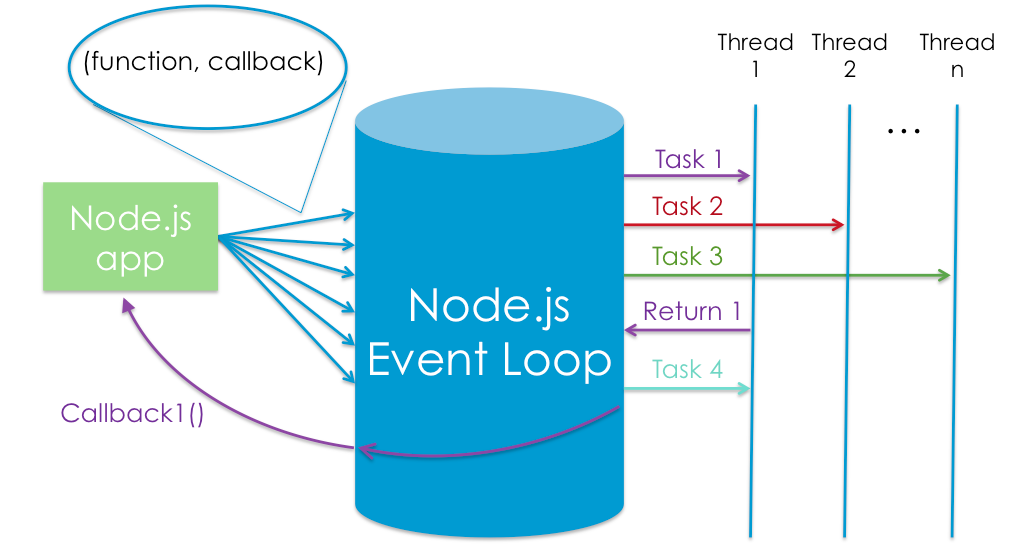
\includegraphics[width=\textwidth,height=\textheight,keepaspectratio]{eventLoop.png} 
\caption{Pętla zdarzeń w środowisku Node.js, źródło: https://stackoverflow.com/ questions/21607692/understanding-the-event-loop}
\end{figure}

\section{Asynchroniczność}
Node.js pracuje wykorzystując tylko jeden wątek, używając technologii asynchronicznego wejścia/wyjścia. 
Zapewnia to synchronizację wykonywania wielu operacji bez konieczności czekania na zakończenie operacji i zwolnienie dostępu do zasobu poprzez zarządzanie żądaniami wejścia/wyjścia w oderwaniu od wątków wykonywania. 
Standardowe operacje synchroniczne powodują zablokowanie dalszego wykonywania wątku do czasu zakończenia przetwarzania. 
W rezultacie określony wątek może zainicjować tylko jedno zadanie wejścia/wyjścia w jednym momencie. 
Wywołanie asynchroniczej funkcji nie czeka na wyniki, dzięki czemu nie blokujemy wątku wykonawczego. 
Po zakończonym wywołaniu uruchomiona zostaje funkcja zwrotna lub ogłoszone zostaje zdarzenie w poszczególnych częściach wykonawczych. 
Pomimo, że Node.js działa na jednym wątku z pętlą zdarzeń, dzięki asynchroniczności potrafi on obsłużyć więcej zapytań niż np. serwer HTTP Apache. 
Uzyskanie wielowątkowości, pomimo korzystania tylko z jednego wątku, jest zapewnione dzięki użyciu wzorca projektowego obserwator, w którym jeden obiekt nazywany przedmiotem obserwowanym określa zależności względem obserwujących go innych obiektów, poprzez wywoływanie ich metod dla określonych własnych stanów. 
W celu obsługi wszystkich asynchronicznych funkcji oraz wątku głównego, Node.js korzysta z biblioteki multiplatformowej języka c - libuv. 
Biblioteka ta została stworzona specjalnie na potrzebny Node.js, ale jest również wykorzystywana w wielu innych technologiach, np. racer: (obsługa serwerów w języku ruby), czy Trevi: (silnik do obsługi aplikacji internetowych w języku swift). 
Wykorzystuje ona określony zbiór wątków do równoległej obsługi wielu operacji wejścia/wyjścia bez wzajemnego ich blokowania. 
Wadą pracy Node.js przy wykorzystaniu tylko jednego wątku jest brak skalowalności pod względem możliwości zwiększenia ilości rdzeni procesorów, na których wykonuje się program, bez użycia dodatkowych modułów, takich jak Cluster (zapewnia możliwość łatwego tworzenia pochodnych procesów, które współdzielą porty serwera), StrongLoop PM (zapewnia zarządzanie procesem produkcyjnym aplikacji Node.js ze wsparciem odpowiedniego zarządzania zasobami, wdrożeniami wielohostowymi oraz interfejsem graficznym), czy PM2 (zarządzanie procesem produkcyjnym, ze wsparciem odpowiedniego zarządzania zasobów, z możliwością nieprzerwanego działania aplikacji przy użyciu przenoszenia jej między domenami, bez potrzeby zatrzymywania pracy). 
Kolejną możliwością na uniknięcie tego ograniczenia jest zmiana ilości wątków należących do zbioru wykorzystywanego przez bibliotekę libuv. 
Wątki te działają na wielu rdzeniach systemu, na którym działa serwer. 
Działanie Node.js jednocześnie na wielu procesach jest zapewnione właśnie dzięki zbiorowi wątków dostarczanych przez bibliotekę libuv.
Wątek główny przydziela zadania dla wątków kolejno ze współdzielonej kolejki funkcji, które wątki pochodne mają za zadanie wykonać. 
Kiedy wątek pochodny zakończy wykonywanie przydzielonego mu zadania, informuje o tym wątek główny poprzez wywołanie określonego wywołania zwrotnego. 
Z przyczyny odpowiedzialności przez watek główny do odebrania wszystkich wywołań zwrotnych, funkcja wykonywana przez jeden wątek pochodny może wstrzymać działanie całej asynchronicznej operacji, a co za tym idzie, zmniejszyć jej całkowitą wydajność. 
Biblioteka libuv zajmuje się odpowiednim podziałem zadań oraz przydzieleniem zasobów tak, aby w jak najlepszy sposób wyważyć nakład pracy między wieloma wątkami. 
\newpage
\begin{figure}[!hb]
\centering
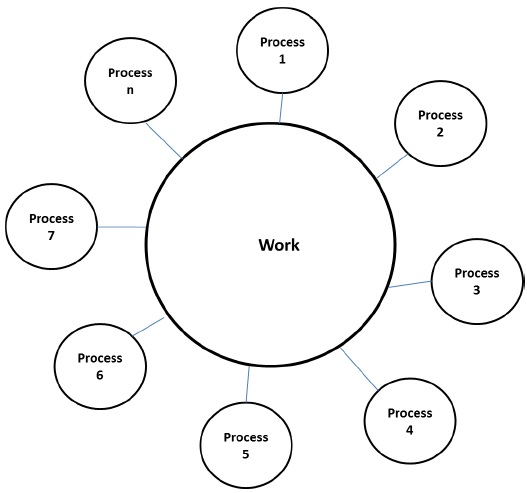
\includegraphics[width=\textwidth,height=\textheight,keepaspectratio]{thread.png} 
\caption{Model programowania współbieżnego wykorzystywany przez Node.js, źródło: www.tutorialspoint.com/parallel\_algorithm/}
\end{figure}

\section{Architektura komunikacji}
W tradycyjnym podejściu odpowiedzialne za obsługę przychodzących połączeń są określone wątki lub procesy sytemu operacyjnego, które w porównaniu z technologią Node.js wymagają względnie więcej zaalokowanych zasobów. 
W celu obsługi zapytania przychodzącego do aplikacji Node.js, program rejestruje się w systemie operacyjnym, aby od każdego przychodzącego połączenia otrzymać odpowiednie wywołanie zwrotne, przez co nie potrzebuje procesów czy wątków, aby uzyskać możliwość obsługi klientów, a tylko własnej pętli głównej, do której wykonywania powraca po przetworzeniu każdego wywołania wstecznego. 
W czasie pracy każde przychodzące połączenie otrzymuje odpowiednią ilość zasobów na stercie programu, więc nie ma również potrzeby alokowania zasobów dla każdego z wątków czy procesów osobno. 
Najbardziej popularna metoda na zarządzanie komunikacją między instancjami korzystającymi z serwera używającego technologii Node.js jest wykorzystanie frameworku Restful Api popularnie zwanego Rest. 
Jest to wzorzec architektury oprogramowania, który opisuje sposób operowania zapytaniami pomiędzy Api, w prosty sposób poprzez obsługę zadań oraz odpowiedzi. 
Został on następnikiem protokołu sieciowego SOAP (Simple object Access protocol), stając się wiodącym standardem. 
Pozwala on na eliminację zbędnej pracy i czasu wymaganego na integrację. 
Daje możliwość na stworzenie komunikacji bez potrzeby wiedzy na temat instancji korzystających z przesyłanych zasobów - może integrować środowiska napisane w różnych językach, działające na różnych platformach. 
Wykorzystuje on proste zapytania przy użyciu protokołu http oraz jego popularnie stosowanych metod takich jak post, get, put, delete, a także bardziej złożonych i używanych rzadziej jak options, head, trace oraz connect. 
Opis typu zasobów, jakie wymieniamy, jest określony w nagłówku informacji przez kod statusu http. 
Poniższa tabelka prezentuje poszczególne typy statusów:
\newpage
\begin{figure}[!hb]
\centering
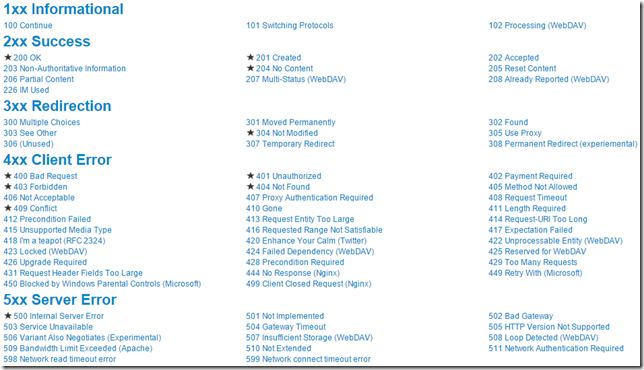
\includegraphics[width=\textwidth,height=\textheight,keepaspectratio]{statuses.png} 
\caption{Kody statusu protokołu http, źródło: http://mokandra.blogspot.fi/2015/10/http-status-code-definitions.html}
\end{figure}

W celu wymiany zasobów framework wykorzystuje najpopularniejsze sposoby opisu struktury służące do opisu obiektów, takie jak najczęściej spotykany, najprostszy w użyciu format json (JavaScript Object Notation) oraz mniej popularny w technologii Rest format xml (eXtensible Markup Language). 
Różnica pomiędzy dwiema formami jest taka, że xml jest językiem niezdefiniowanych znaczników, a json tylko sposobem na prezentację właściwości obiektu. 
Porównanie obydwu struktur:
Struktura w formacie json opisująca listę pracowników:
\begin{lstlisting}[language=json,firstnumber=1]
{"employees":[
	{ "firstName":"James", "lastName":"Bond" },
	{ "firstName":"David", "lastName":"Klint" },
	{ "firstName":"Peter", "lastName":"Blom" }
]}
\end{lstlisting}
\newpage
Ta sama struktura opisana w formacie xml:
<employees>
\begin{lstlisting}[language=XML,firstnumber=1]
	<employee>
		<firstName>James</firstName> <lastName>Bond</lastName>
	</employee>
	<employee>
		<firstName>David</firstName> <lastName>Klint</lastName>
	</employee>
	<employee>
		<firstName>Peter</firstName> <lastName>Blom</lastName>
	</employee>
</employees>
\end{lstlisting}

\section{Alternatywne rozwiązania}
\subsection{Vert.x}
Pierwszą alternatywą dla technologii Node.js jest framework Vert.xm.
Pracuje on na środowisku JVM (Java Virtual Machine) i tak jak i Node.js, jest środowiskiem sterowanym zdarzeniami.
Został napisany w 2011 roku przez zainspirowanego technologią Node.js Tim Foxa przy użyciu między innymi języków Java, JavaScript, Python, Ruby.
Dzięki platformie JVM aplikacje mogą być stworzone dla wielu systemów operacyjnych.
Wykorzystuje on niskopoziomową bibliotekę Netty, służącą do asynchronicznej obsługi urządzeń wejścia/wyjścia w celu obsługi aplikacji w architekturze klient-serwer.
Do wytwarzania oprogramowania w Vert.x możemy użyć różnych języków programowania - Java, Javascript, Groovy, Ruby, Ceylon, Scala lub Kotlin.
Jest więc dobrą alternatywą w przypadku potrzeby użycia języka innego niż javascript.
Potrafi on szybciej od technologii Node.js odpowiedzieć na proste żądania, natomiast jest mniej efektywny na przykład przy pracy z gniazdami sieciowymi.

\subsection{Twisted}
Kolejną alternatywą dla technologii Node.js jest framework Twisted.
Został stworzony w 2002 roku przez Glyph Lefkowitz'a przy użyciu technologii Python.
Wspiera koncepcje środowiska sterowanego zdarzeniami, więc nie wymaga tworzenia osobnych wątków dla obsługi wielu procesów w jednym czasie. 
Do procesu wytwarzania oprogramowania przy jego użyciu niezbędna jest umiejętność pisania w języku python.
Działanie framework'u twisted opiera się głównie na wykorzystaniu protokołów sieciowych, między innymi HTTP, XMPP, TCP, IMAP, SSH czy Udp.
Dzięki długiemu okresu rozwoju framework oferuje wsparcie wielu rozwiązań sieciowych.
Nie oferuje tak efektywnej pracy jak technologia Node.js, jednak może okazać się lepszym wyborem, jeśli zachodzi potrzeba wykorzystania specyficznego protokołu sieciowego, który nie został jeszcze zaimplementowany w Node.js.

\subsection{Ringojs}
Ostatnią wymienioną alternatywą jest platforma Ringojs.
Napisany został w języku java przez Hannesa Wallnöfer w 2010 roku.
Służy do tworzenia aplikacji w języku javascript po stronie serwera działających również w koncepcji środowiska sterowanego zdarzeniami dzięki wykorzystaniu technologii Rhino, która zajmuje się obsługą wielowątkowości. 
Niewątpliwą zaletą Ringojs jest możliwość wykorzystania kodów w języku java przez serwer, zapewniając integracje frameworka z istniejącymi środowiskami java'owymi.
W porównaniu z technologią Node.js, Ringojs jest efektywniejszy dla rozwiązań obsługujących mniejszą ilość jednoczesnych zapytań, oraz w przypadku alokacji dużych plików
dzięki pracy w środowisku JVM. 
Oznacza to, że zyskuje przewagę w przypadku prostych narzędzi, natomiast nie gwarantuje takiej skalowalności jak Node.js.

\chapter{Założenia i specyfikacja aplikacji}

\section{Specyfikacja problemu}
Potrzebny jest nowoczesny system do zarządzania tablicami zadań, który będzie posiadał autoryzowany dostęp dla użytkowników systemu. 
Został zauważony problem braku prostej w obsłudze, intuicyjnej aplikacji pozwalającej we współpracy z innymi użytkownikami na zarządzanie zarówno podziałem jak i procesem realizacji wyszczególnionych zadań.
W celu reakcji na zapotrzebowanie zostanie zaprojektowany system informatyczny, pracujący w technologii Node.js, ze względu na możliwą do osiągnięcia niezawodność oraz dostępność nawet przy jednoczesnej obsłudze wielu korzystających z aplikacji klientów.
Nie powinien on wymagać żadnych procesów wdrożeniowych w celu zrozumienia obsługi narzędzia, ponieważ celem projektu jest stworzenie narzędzia, które wspiera, a nie dodatkowo komplikuje określone zadania.
System powinien w przejrzysty sposób prezentować proces realizacji poszczególnych zadań zorganizowanych w tablicach.
Właściciel określonej tablicy powinien mieć możliwość zarządzania dostępem do tablicy poprzez udostępnianie lub ograniczanie jej treści pozostałym użytkownikom.
Aplikacja zapewni subskrybentom nieprzerwaną możliwość nadzoru, wglądu oraz określania aktualnych statusów dowolnych procesów.
\newpage
\section{Wymagania funkcjonalne}
Analiza wymagań funkcjonalnych umożliwia zidentyfikowanie i opisanie pożądanego zachowania systemu. 
Umożliwiają określenie usług oferowanych przez system, reakcji na dane wejściowe oraz zachowania w określonych sytuacjach.
\begin{itemize}
\item Wymiana komunikatów w modelu klient-serwer.
\item Możliwość utworzenia do 1000000 kont użytkowników.
\item Możliwość zmiany danych użytkownika.
\item Weryfikacja adresu email przed aktywacją.
\item Możliwość resetowania hasła za pomocą adresu email.
\item Utrzymanie do 100 tablic jednocześnie dla użytkownika.
\item Możliwość usuwania tablic.
\item Obsługa do 1000 równoległych członków jednej tablicy.
\item Możliwość zarządzania członkami tablicy.
\item Obsługa do 10000 równoległych zadań dla tablicy.
\item Możliwość usuwania zakończonych zadań.
\item Utrzymanie do 1000 statusów do jednego zadania.
\item Zapamiętywanie terminu zmiany statusu zadań.
\item Walidacja poprawności wprowadzanych przez użytkownika danych zarówno po stronie klienta jak i serwera.
\item W razie wystąpienia nieprawidłowych danych system powiadamia o błędach.
\item Zapewnienie okna pomocy opisującego korzystanie z aplikacji.
\item Możliwość otrzymywania powiadomień o aktualnym statusie tablic oraz poszczególnych zadań.
\item System współpracuje z bazą danych.
\end{itemize}

\section{Wymagania pozafunkcjonalne}
Wymagania niefunkcjonalne opisują kryteria umożliwiające dokonanie oceny działania systemu i elementów mających wpływ na satysfakcję użytkownika.
Zdefiniowane zostały następujące wymagania niefunkcjonalne:

\begin{itemize}
\item Dostęp do określonych zasobów musi być chroniony poprzez login i hasło użytkownika.
\item Budowa interfejsu użytkownika musi być możliwie intuicyjna i prosta w obsłudze.
\item Proste analizowanie i diagnozowanie błędów oraz sytuacji problemowych.
\item Budowa zapewnia łatwe wprowadzanie koniecznych zmian.
\item Jest w stanie obsłużyć jednocześnie do 100.000 użytkowników.
\item Czas uruchomienia jest nie dłuższy niż 10 sekund.
\item Umożliwia efektywne testowanie wprowadzonych zmian.
\item Posiada możliwość obsługi poprzez różne przeglądarki internetowe i środowiska.
\item Zrozumiały dla wszystkich. Czas przyswojenia nie przekracza 15 minut.
\item Ma możliwość współistnienia z innymi modułami.
\item Spełnia wszystkie normy prawne w naszym kraju.
\end{itemize}
\newpage
\section{Diagram przypadków użycia}
Poniższy diagram uml przedstawia schemat użytkowania systemu.
Określone zostały trzy poziomy klientów korzystających z aplikacji, które określają zakres udostępnionej funkcjonalności.

\begin{figure}[!hb]
\centering
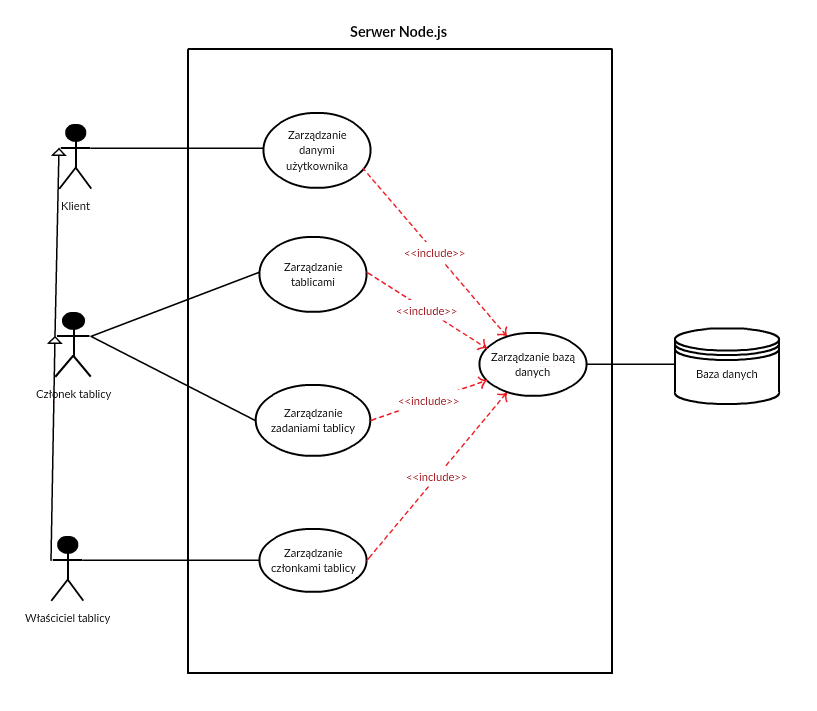
\includegraphics[width=\textwidth,height=\textheight,keepaspectratio]{SCHEME.png}
\caption{Diagram przypadków użycia, źródło: Opracowanie własne}
\end{figure}

\chapter{Opracowanie aplikacji}

\section{Mean Stack}

\subsection{Wstęp}
Do opracowania rozwiązania zdecydowałem się skorzystać z Mean Stack. 
Skrót odnosi się do frameworków oraz technolgii Mongodb, Express, AngularJS oraz Node.js. 
Współpracując razem zapewniają bardzo szybkie, efektywne tworzenie skalowalnych aplikacji wieloplatformowych. 
Do użycia wszystkich wymagany jest tylko jeden język programowania - javaScript, zarówno do obsługi warstwy frontendowej aplikacji jak i backendowej. 
Wszystkie technologie są dostępne w pełni bezpłatnie. 

Jako iż Technologia Node.js została już opisana, przejdę do opisu pozostałych technologii.

\subsection{MongoDB}
Napisany w języku c++ system zarządzania bazą danych zorientowany na dokumenty. 
Operuje na nierelacyjnych bazach danych. 
Używa struktur json jako schematów budowy bazy danych.
Udostępnia całkowitą dowolność w budowie struktury wymaganej bazy danych. 
Wykorzystuje proste, ale zapewniające szerokie możliwości zapytania bazodanowe.

\subsection{ExpressJS }
Framework służący do szybkiego wymagającego jak najmniejszych nakładów pracy wytwarzania zarówno backendu aplikacji internetowych, jak i aplikacji mobilnych.
Dostarcza zbiór określonych klas i metod. Jest to najpopularniejszy framework do tworzenia serwerów w technologii Node.js.

\subsection{AngularJS}
Wykorzystujący wzorzec projektowy MVC (Model View Controler) polegający na oddzieleniu od siebie poszczególnych warstw aplikacji - logiki, widoku oraz modelu komunikacji, framework wykorzystujący dodatkowe tagi w języku html w celu prostego w obsłudze i niewymagającego dodatkowej logiki napisanej w języku javaScript tworzenia dynamicznych stron internetowych.

\section{Komunikacja}

\subsection{Rozwiązanie problemu komunikacji}
Do komunikacji między warstwą frontendową i backendowową po stronie klienta wykorzystałem wysokopoziomową bibliotekę Ajax oraz technologię Restful api. 
Ajax polega na zarządzaniu asynchroniczną komunikacją. 
Dzięki temu aplikacja może wykonywać inne funkcje, mimo oczekiwania na odpowiedź ze strony serwera, za sprawą odseparowania warstwy wymiany danych od pozostałych warstw aplikacji.
Do opisu wymienianych struktur użyłem standardu json, ponieważ wymaga on mniejszych nakładów pracy od standardu xml. 
Powyższe frameworki współpracują ze sobą w bardzo intuicyjny i przejrzysty sposób. 
Angular prezentuje użytkownikowi dynamiczną aplikację internetową, odpowiada za przyjmowanie danych i z pomocą ajaxa wysyła oraz odbiera dane wysyłane do serwera. 
Serwer Node.js z użyciem technologii express, wykorzystując metodę routingu, dopasowuje zapytanie do odpowiednich funkcji serwisu, przetwarza otrzymane dane, przy współpracy z bazą danych zarządzana przez Mongodb przechowuje informacje użytkowników serwisu oraz w odpowiedzi zwraca odpowiednie dane z powrotem do warstwy frontendowej prezentującej dane użytkownikowi. 
\newpage
\begin{figure}[!hb]
\centering
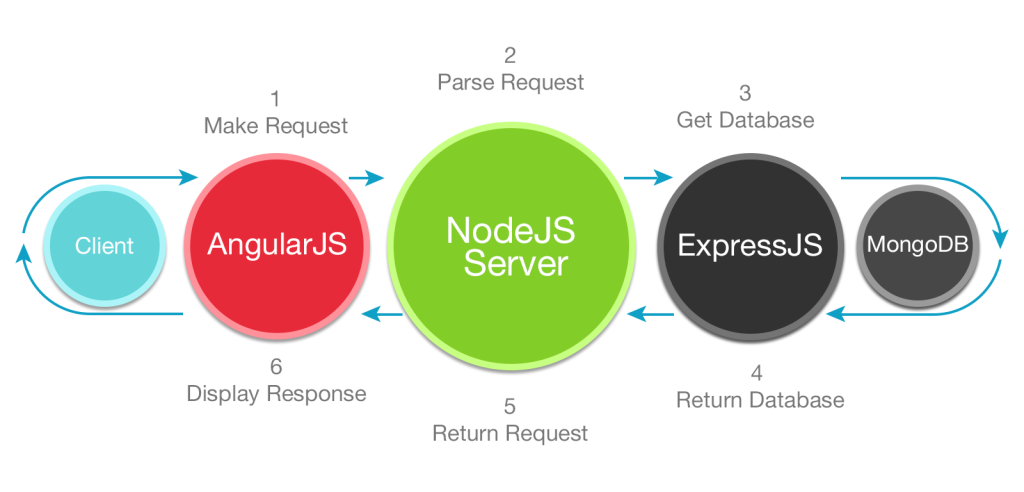
\includegraphics[width=\textwidth,height=\textheight,keepaspectratio]{Meanex.png}
\caption{Przepływ komunikacji w MEAN Stack, źródło: https://www.dealfuel.com/seller/mean-stack-tutorial/}
\end{figure}

\subsection{Schematy wymiany zasobów}
Uniwersalny dla aplikacji schemat procesu pobrania statycznych zasobów z serwera wykorzystuje metodę get. Do zasobów tych należy między innymi plik html, zawierający warstwę prezentacji aplikacji, plik css zawierający styl warstwy prezentacji, czy plik zawierający funkcje wykorzystywane przez aplikacje w języku javaScript. Proces prezentuje się następująco:
\begin{figure}[!hb]
\centering
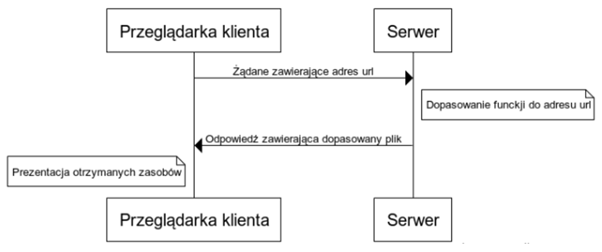
\includegraphics[width=\textwidth,height=\textheight,keepaspectratio]{K-S.png} 
\caption{Pobranie statycznych zasobów, źródło: Opracowanie własne}
\end{figure}
\begin{enumerate}
\item Klient przy użyciu przeglądarki wysyła pod określony adres url serwera zapytanie zawierające pożądany zasób.
\item Serwer otrzymuje zapytanie i dopasowuje określoną funkcję po adresie url serwera.
\item Funkcja wybiera dopasowane do zapytania zasoby i wysyła odpowiedź do aplikacji.
\item Aplikacja odbiera i zaczyna korzystać z zasobów.
\end{enumerate}

 Uniwersalny dla aplikacji schemat procesu wymiany danych określonych dla specyficznego użytkownika wykorzystuje metodę post. Przykładowe dane wymieniane przez aplikacje to login, hasło, informacje odnośnie żądań użytkownika, komentarze do zadań użytkownika. Przepływ danych wygląda następująco:
 \begin{figure}[!hb]
\centering
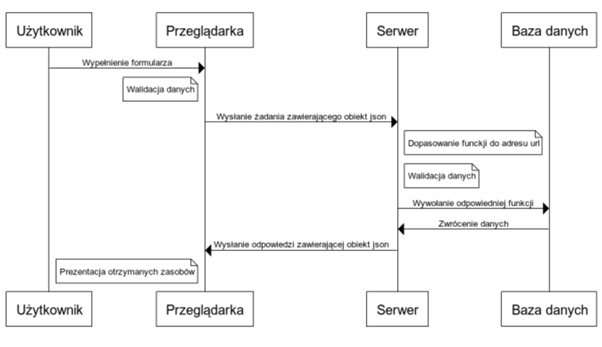
\includegraphics[width=\textwidth,height=\textheight,keepaspectratio]{U-P-S-B.png} 
\caption{Wymiana zasobów w formacie Json źródlo: Opracowanie własne}
\end{figure}
\begin{enumerate}
\item Dane zostają pobrane od użytkownika w określonym formularzu w warstwie frontendowej.
\item Dane zostają zwalidowane pod kątem poprawności po stronie użytkownika.
\item Jesli dane są poprawne, zostają zorganizowane w obiekcie json i wysłane do serwera, w przeciwnym wypadku zostaje zwrócony błąd.
\item Serwer odbiera zapytanie i przekazuje je do odpowiedniej funkcji.
\item Dane zostają zwalidowane pod kątem poprawności po stronie serwera.
\item Jeśli dane są poprawne, serwer realizuje określoną funkcję przy pomocy zapytań bazodanowych, w przeciwnym wypadku zostaje przygotowany komunikat o błędzie.
\item Odpowiedź na zapytanie bazodanowe zostaje odebrana i zostają przygotowane dane do wysłania.
\item Przygotowane dane zostają wysłane w określonej odpowiedzi.
\item Warstwa frontendowa otrzymuje odpowiedź i zostaje odświeżona warstwa prezentacji aplikacji.
\end{enumerate}
 

\subsection{Kod po stronie klienta wysyłający żądanie}
Przykładowy kod wykonywany po stronie klienta, wysyłający żądanie do serwera, żądające określonego zasobu przy użyciu frameworku Angularjs:
Plik w języku javaScript zawierający definicje modelu i kontrolera:
\medskip
\begin{lstlisting}
var main = angular.module("main", []); 									// create angular module

main.controller('SignInController', function($scope) { 					// create controller for module
	$scope.SignIn=function(){ 											// callback function as field in model
		if ($scope.login && $scope.password) {							// if both field are filled
			var xhr = new XMLHttpRequest();									//create request object
			xhr.open("POST", http://site.com/authorization, true);		// set method type, domain address and is it asynchronous
			xhr.setRequestHeader("Content-type","application/json");	// set header with information of content type
			req.send(JSON.stringify({	login: $scope.login,			
										password: $scope.password})); 	// Send json object with login and password
			req.onreadystatechange = function() { 						// create callback, called on every state change
				if (req.readyState === 4) { 							// readyState 4 is 4 when respond is got
					if (req.status === 200) { 							// http status code 200 - ok
						var resObj = JSON.parse(this.responseText);		// parse response text to json object
						$scope.login=resObj.login;						// set password from response
						$scope.password=$resObj.password;				// set password from response
						alert("Login and password are valid");			// alert user
					}
					else{ 												// all other http statusses
						alert(req.status+":"req.responseText); // alert user
					}
				}
			}
		}
	}
}
\end{lstlisting}
\newpage
Plik w języku html zawierający definicję widoku:
\begin{lstlisting}[language=HTML]
<!DOCTYPE html> 
<!-- Apply view to model -->
<body ng-app = "main">
	<!-- Create form for request -->
	<form class="main" name="form"> 
		<!-- Get user login -->
		<input type = "text" ng-model = "login" name="login"
			<!-- Set field validation -->
			required ng-pattern='/^[a-zA-Z0-9._-]+$/'  ng-maxlength="20" ng-minlength="3">
		<!-- Get user password -->
		<input type = "text" ng-model = "password" name="password"
		<!-- Set field validation -->
			required ng-pattern='/^[a-zA-Z0-9._-]+$/'  ng-maxlength="20" ng-minlength="3">
	</form>
</body>
\end{lstlisting}

\subsection{Kod po stronie serwera obsługujący odebranie żądania}
Przykładowy kod, wykonywany po stronie serwera, obsługujący odebrane żądanie od klienta przy użyciu technologii Node.js oraz frameworków express i mongodb:
\medskip
\begin{lstlisting}
var express = require('express');					// load express module
var bodyParser = require('body-parser');    		// load module for parsing json data
var dataBase = require('mongodb').MongoClient;  	// load MongoDB database module
var Promise = require('promise');               	// load asynchronous returns from functions module

var app = express();						        // create epress configuration object
app.use(bodyParser.json());                         // load bodyParser to app object

// check if database contains given user
var Authorization=function (login, password) {
    return new Promise(function (fulfill, reject) {
        dataBase.connect(mongodb://localhost:27017/db, function(err, db).done(function (db) {
            db.collection("Users").findOne({ login: login, password: password }, function (err, result) {
                if (result != null) {
                    fulfill(true);
                }
                else {
                    fulfill(false);
                }
                db.close();
            });
        });
    });
}

// check is text format correct
function TextValidation(text, min, max) {
    if (min === undefined) min = 0;
    if (max === undefined) max = Infinity;
    return (text !== undefined) && (/(^[a-zA-Z0-9._-]+$){min, max}/).test(text);
}

// check is user credentials data correct
function UserValidation(body) {
    return new Promise(function(fulfill, reject) {
        if (!TextValidation(body.login, 3, 20) || !TextValidation(body.password, 3, 20)) {
            fulfill(false);
            return;
        }
        Authorization(body.login, body.password).done(function (authentication) {
            fulfill(authentication);
        });
    });
}

//funtion run when server gets post request with url /authorization
app.post('/authorization', function (req, res) {
	UserValidation(req.body).done(function(valid) {
		res.setHeader('Content-Type', "text/html");
	    if (valid) {
			res.statusCode = 200;
	   	}
        else {
			res.statusCode = 401; // error has happend
			res.write("Invalid login or password");
		}
		res.end();
    });
});

//start server
var server = app.listen(8081, function () {});
\end{lstlisting}

\section{Wykorzystane moduły}

\subsection{Moduły zewnętrzne}
Zewnętrzne moduły, zainstalowane za pomocą zbioru repozytorium npm, które użyłem do realizacji rozwiązania, to:
\begin{enumerate}
\item express - opisany powyżej
\item fs - file stream, odpowiada za obsługę zapisu oraz wczytywania plików. 
Wykorzystywany w celu wczytywania plików statycznych aplikacji, takich jak index.htm (strona główna w formacie html), main.js (funkcje w języku javaScript), style.css (plik arkuszu stylów, odpowiadający za styl prezentacji), favicon (ikona serwisu wyświetlana w oknie przeglądarki), czy losowo wybieranych zdjęć wyświetlanych w tle serwisu.
\item path - obsługa różnic między systemami operacyjnymi. 
Dzięki temu modułowi możemy zapewnić całkowitą sprawność naszego serwisu, niezależnie od środowiska uruchomieniowego. 
Pozwala niwelować różnice w lokalizacji plików systemowych, czy łącznikach pomiędzy poszczególnymi folderami przy specyfikacji ścieżki do pliku.
\item body-parser - dostarcza możliwość analizowania danych, załączonych do odebranego przez serwer żądania, wykorzystany został w celu odczytu poszczególnych wartości odebranych w formacie json.
\item promise - odpowiada za operowanie wynikami otrzymanymi w wyniku asynchronicznych funkcji. 
Dzięki temu modułowi nie musimy synchronicznie czekać na otrzymanie zwrotu z kolejnych funkcji, natomiast możemy przy użyciu wywołań zwrotnych zareagować po otrzymaniu określonego wyjścia.
\item cookie-parser - zapewnia możliwość wykorzystania plików cookie dla specyficznego klienta. 
Dzięki temu modułowi możemy ustawiać, usuwać lub edytować wartości plików cookie, które zostaną przydzielone dla konkretnego użytkownika w ramach całej sesji komunikacji z użytkownikiem lub przez określony przez nas czas. 
\item request - dostarcza możliwość wysyłania prostych zapytań http pod wskazany adres zawierających strukturę w formacie json oraz odebranie na nie odpowiedzi. 
Moduł został użyty wyłącznie do testów aplikacji.
\end{enumerate}

\subsection{Moduły wewnetrzne}
Wewnętrzne moduły, czyli takie, które zostały napisane przeze mnie specjalnie na użytek projektu, to:
\begin{enumerate}
\item db.js (wykorzystujący zewnętrzny moduł mongodb) - moduł zapewnia komunikację z bazą danych w technologii mongodb, poprzez wywoływanie odpowiednich funkcji. 
Został dostosowany bezpośrednio do obsługi bazy danych dla wykonywanego projektu. 
Dzięki temu plik główny serwera nie musi znać budowy, ani wykonywać operacji bezpośrednio na dokumentach bazy danych.
\item emails.js (wykorzystujący zewnętrzny moduł nodemailer) - dostarcza obsługę wysyłania wiadomości email do użytkowników serwisu w przypadku zajścia określonych sytuacji, takich jak na przykład otrzymanie nowego zaproszenia czy zmiana statusu zadania. Moduł dostarcza jedną, prostą w obsłudze funkcję zapewniającą obsługę wiadomości email. 
\end{enumerate}


\chapter{Testy aplikacji}
Na wykonanej aplikacji zostały wykonane poniższe testy, sprawdzające poprawność dostarczanej przez serwis funkcjonalności.
Do testów została użyta przeglądarka Google Chrome oraz skrypty node.js korzystające z modułu request.
Bardziej zaawansowaną technologią do testowania aplikacji webowych jest framework Selenium, pozwalający na automatyzacje testów. 
Dostarcza on możliwość nagrania lub zaprogramowania określonego testu, a po jego odegraniu sprawdzania przychodzące odpowiedzi lub reakcję aplikacji.

\newpage
\section{Testy manualne}
\subsection{Uzyskanie dostępu do statycznych zasobów serwisu}
\begin{figure}[!hb]
\centering
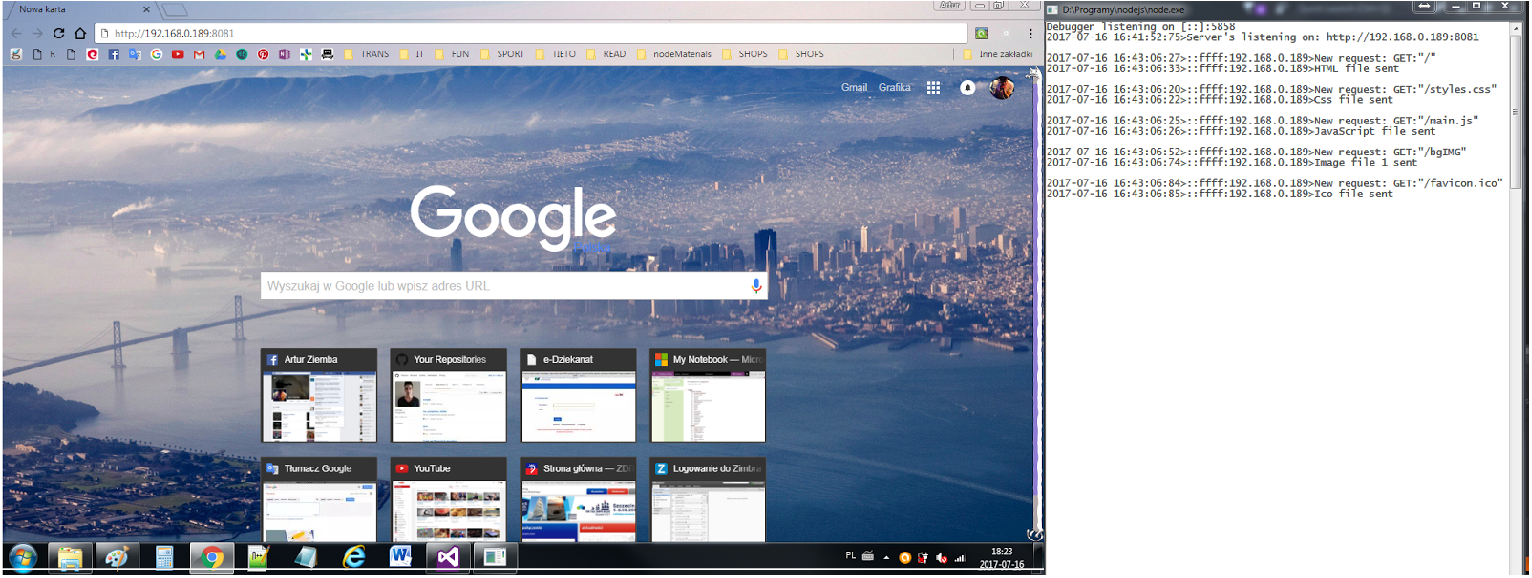
\includegraphics[width=\textwidth,height=\textheight,keepaspectratio]{12.png}
\captionsetup{labelformat=empty}
\caption[]{Użytkownik wysyła żądanie pod adres serwera. 
Otrzymuje odpowiedź zawierającą pliki statyczne serwisu (plik html, css, js, zdjęcie w tle i favicon.}
\end{figure}

\subsection{Rejerstracja w serwisie}
\begin{figure}[!hb]
\centering
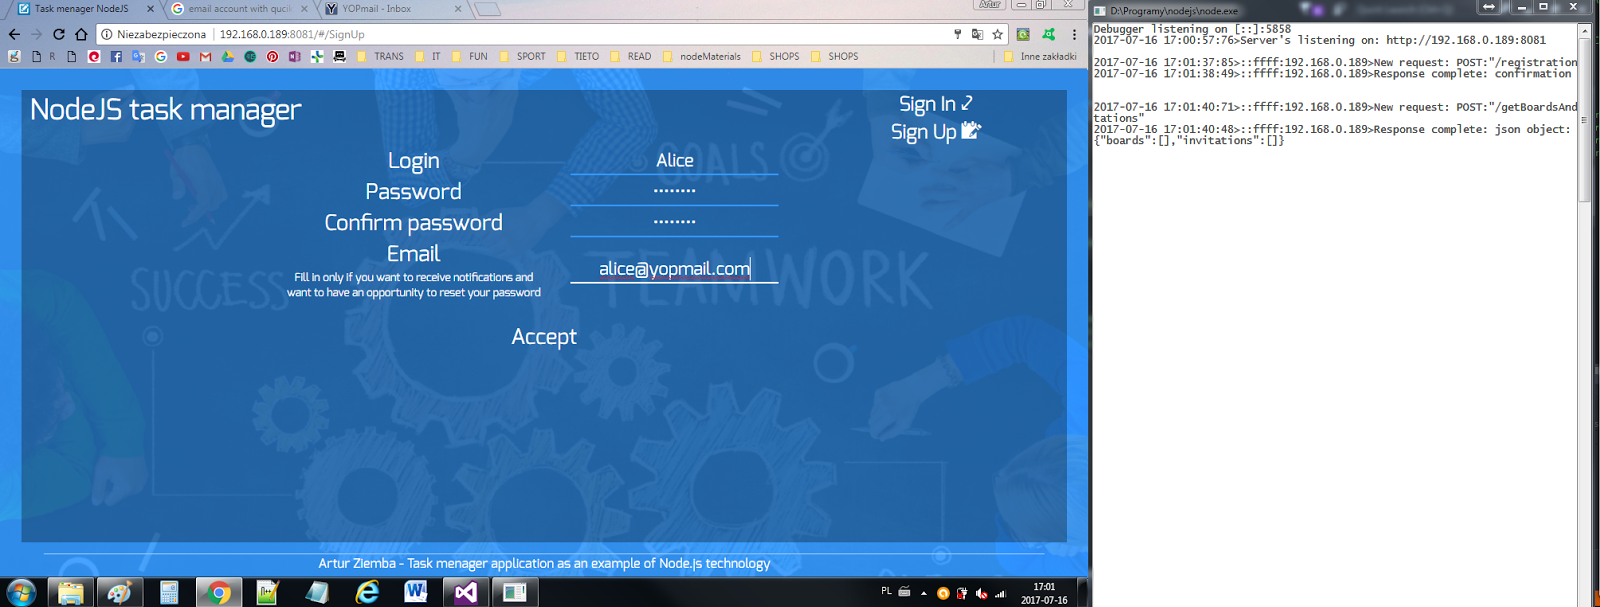
\includegraphics[width=\textwidth,height=\textheight,keepaspectratio]{22.png}
\captionsetup{labelformat=empty}
\caption[]{Użytkownik wypełnia formularz rejestracyjny na stronie serwisu i wysyła dane do serwera. 
Serwer sprawdza poprawność otrzymanych danych i w odpowiedzi przesyła stronę główną aplikacji dostępną po zalogowaniu na konto lub informacje o błędzie.}
\end{figure}

\subsection{Potwierdzenie adresu email}
\begin{figure}[!hb]
\centering
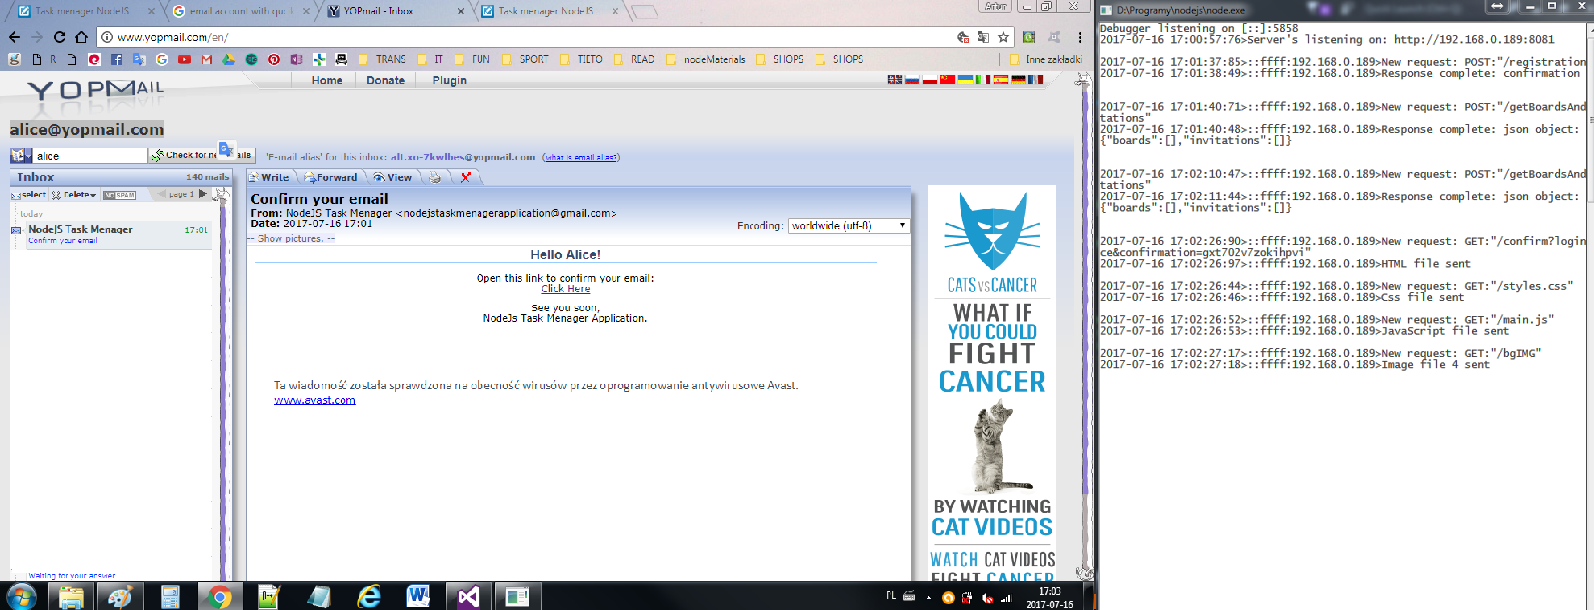
\includegraphics[width=\textwidth,height=\textheight,keepaspectratio]{32.png}
\captionsetup{labelformat=empty}
\caption[]{Po podaniu adresu email użytkownik otrzymuje wiadomość email zawierającą link aktywacyjny. 
Po kliknięciu w link. Serwer sprawdza czy otrzymany w linku kod jest prawidłowy dla podanego użytkownika. 
Następnie aktywuje adres email dla odpowiedniego użytkownika, wysyła w odpowiedzi stronę główną aplikacji oraz wiadomość email o potwierdzeniu.}
\end{figure}

\newpage 
\subsection{Logowanie się w serwisie}
\begin{figure}[!hb]
\centering
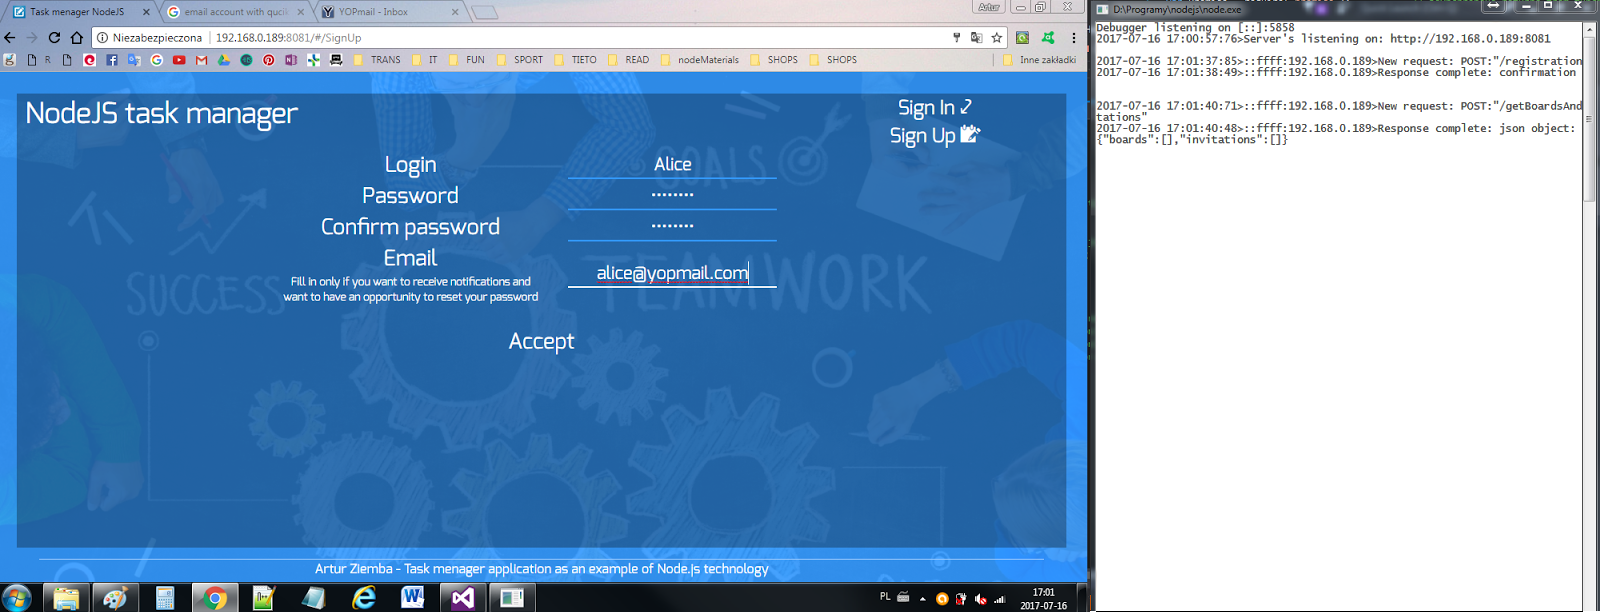
\includegraphics[width=\textwidth,height=\textheight,keepaspectratio]{42.png}
\captionsetup{labelformat=empty}
\caption[]{Użytkownik wypełnia formularz na stronie serwisu i przesyła żądanie do serwera. Serwer sprawdza istnienie konta w serwisie. 
W odpowiedzi użytkownik otrzymuje stronę główną aplikacji lub błąd o niepoprawnych danych.
W czasie bycia zalogowanym, co określony czas zostaje wysłane żądanie aktualizacji danych. 
Aktualizacja następuje również każdorazowo po otrzymaniu pomyślnego potwierdzenia wykonania operacji przez serwer.}
\end{figure}

\newpage 
\subsection{Resetowanie hasła użytkownika}
\begin{figure}[!hb]
\centering
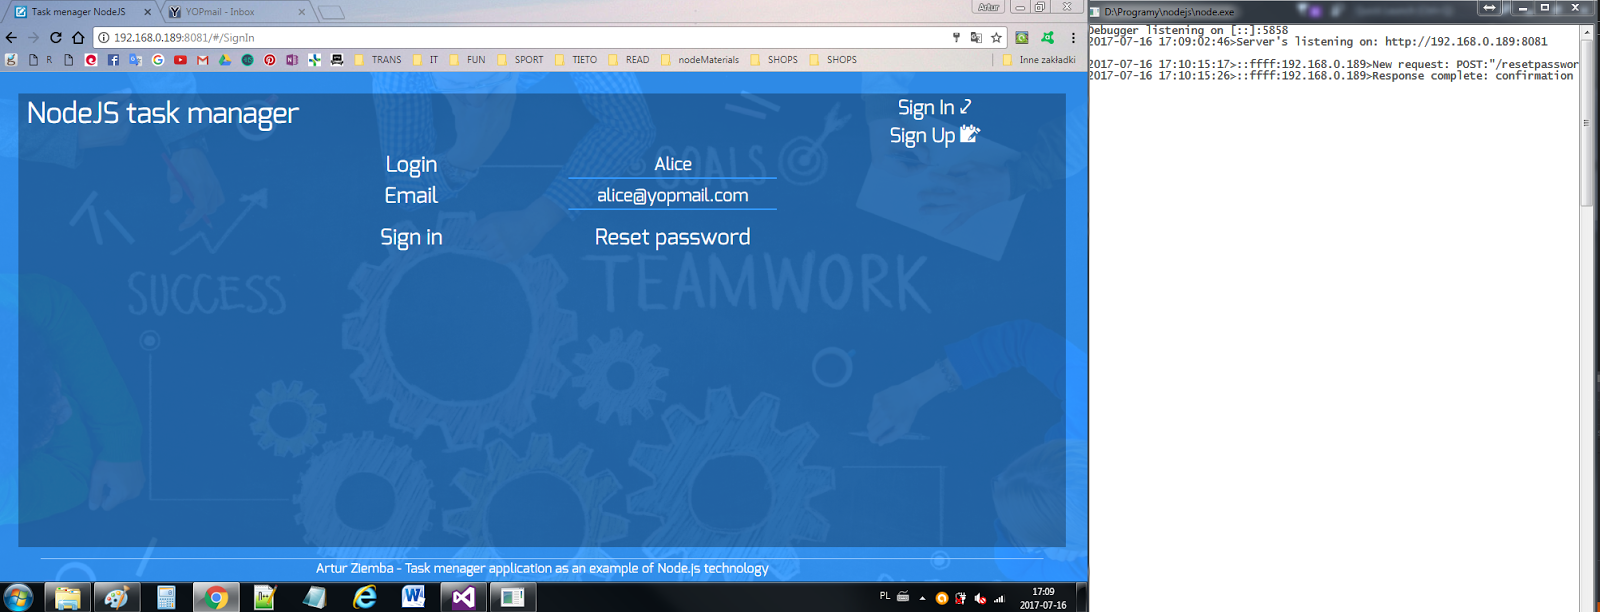
\includegraphics[width=\textwidth,height=\textheight,keepaspectratio]{52.png}
\captionsetup{labelformat=empty}
\caption[]{Funkcja jest dostępna po potwierdzeniu adresu email dla konta. 
Po wypełnieniu odpowiedniego formularza na stronie głównej serwisu, użytkownik wysyła żądanie do serwera. 
Serwer sprawdza podane dane. W odpowiedzi wysyła informacje o przetworzeniu żądania.}
\end{figure}
\begin{figure}[!hb]
\centering
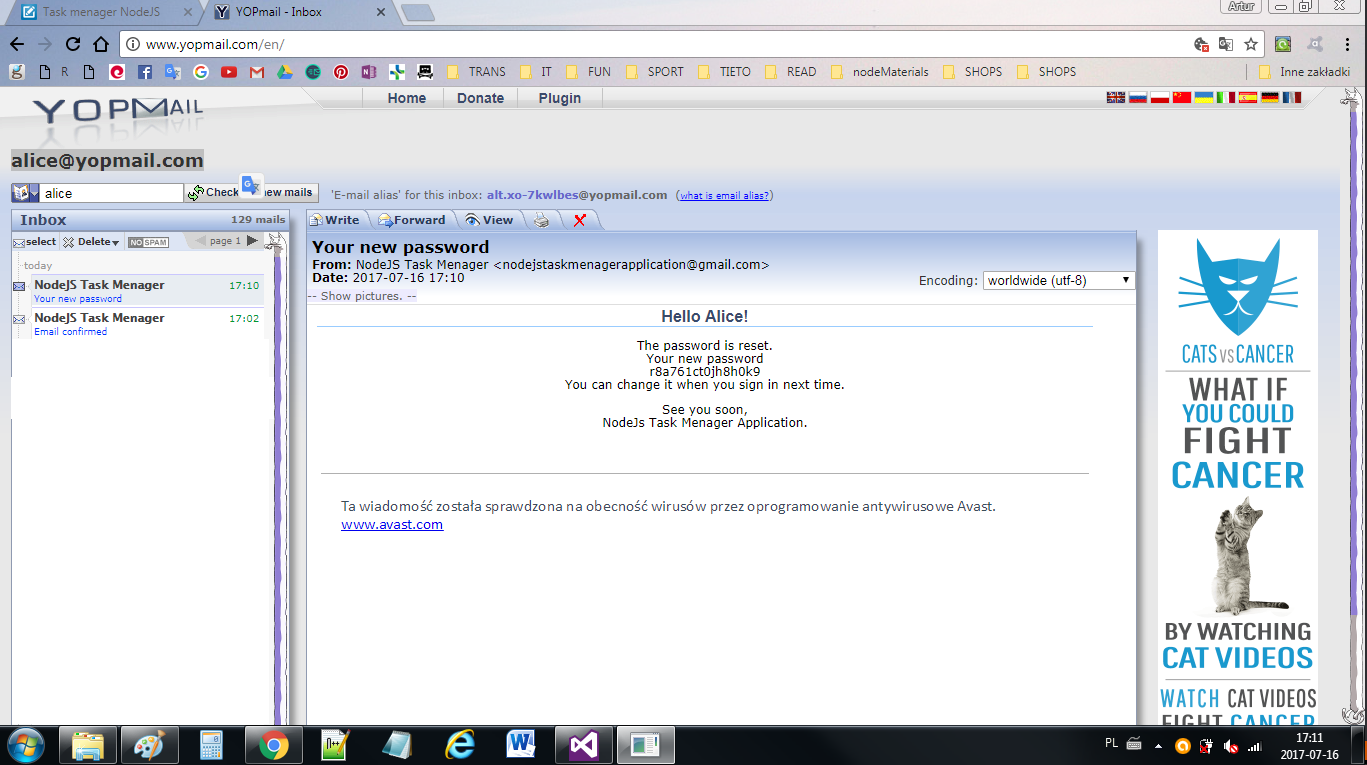
\includegraphics[width=\textwidth,height=\textheight,keepaspectratio]{53.png}
\captionsetup{labelformat=empty}
\caption[]{Otrzymujemy także wiadomość email zawierającą nowe hasło do serwisu.}
\end{figure}

\newpage 
\subsection{Zmiana danych użytkownika}
\begin{figure}[!hb]
\centering
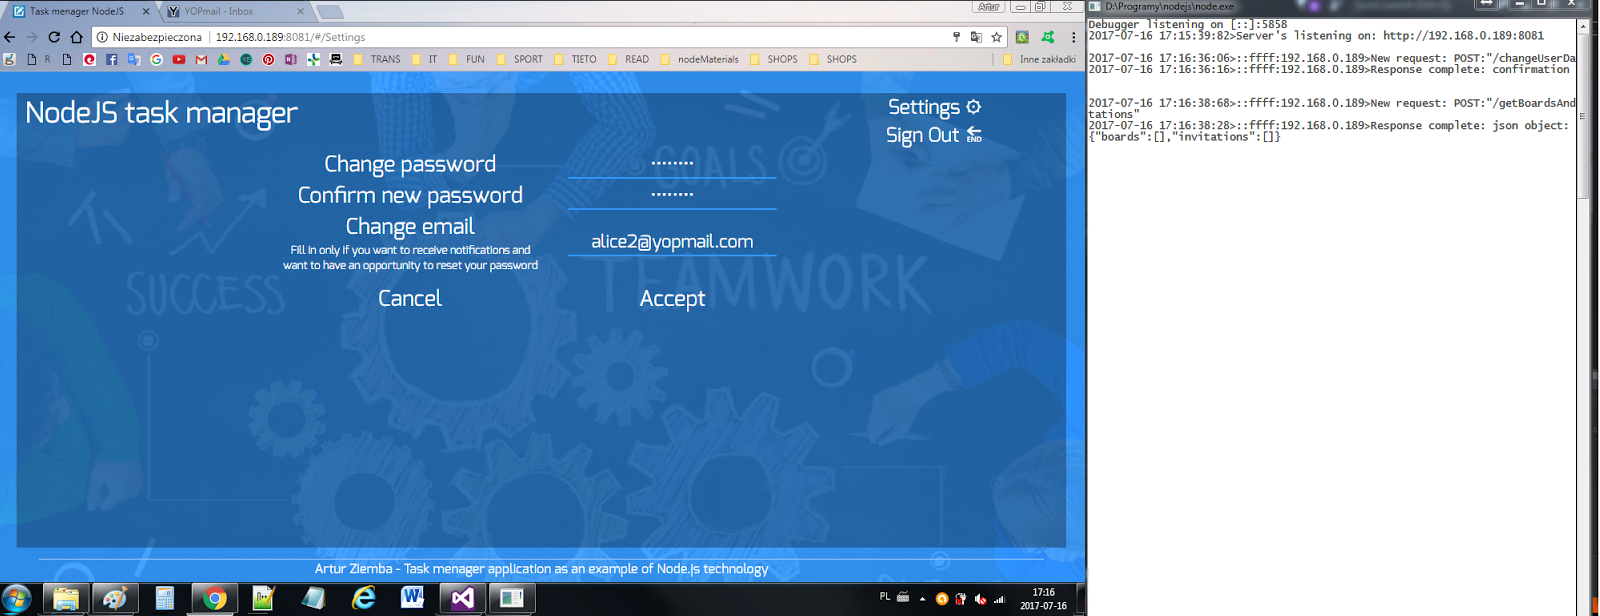
\includegraphics[width=\textwidth,height=\textheight,keepaspectratio]{62.png}
\captionsetup{labelformat=empty}
\caption[]{Po zalogowaniu się i wypełnieniu odpowiedniego formularza na stronie serwisu użytkownik wysyła żądanie do serwera. 
Serwer sprawdza poprawność danych. Jeśli są poprawne, aktualizuje je.
W przeciwnym wypadku, zwraca komunikat o błędzie. 
W odpowiedzi serwer wysyła stronę główną aplikacji.}
\end{figure}
\begin{figure}[!hb]
\centering
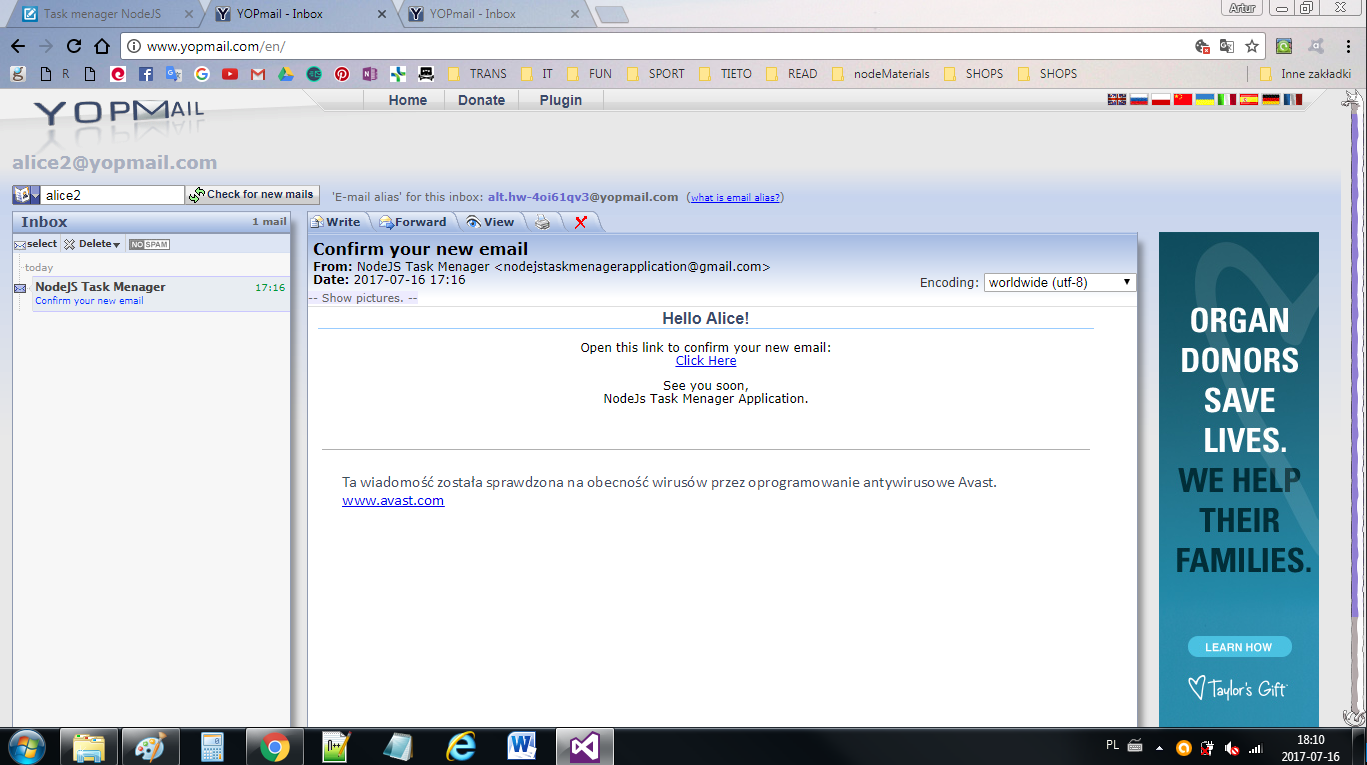
\includegraphics[width=\textwidth,height=\textheight,keepaspectratio]{63.png}
\captionsetup{labelformat=empty}
\caption[]{Jeśli zmieni się również adres email, użytkownik musi go ponownie zweryfikować. }
\end{figure}

\newpage 
\subsection{Utworzenie nowej tablicy z zadaniami}
\begin{figure}[!hb]
\centering
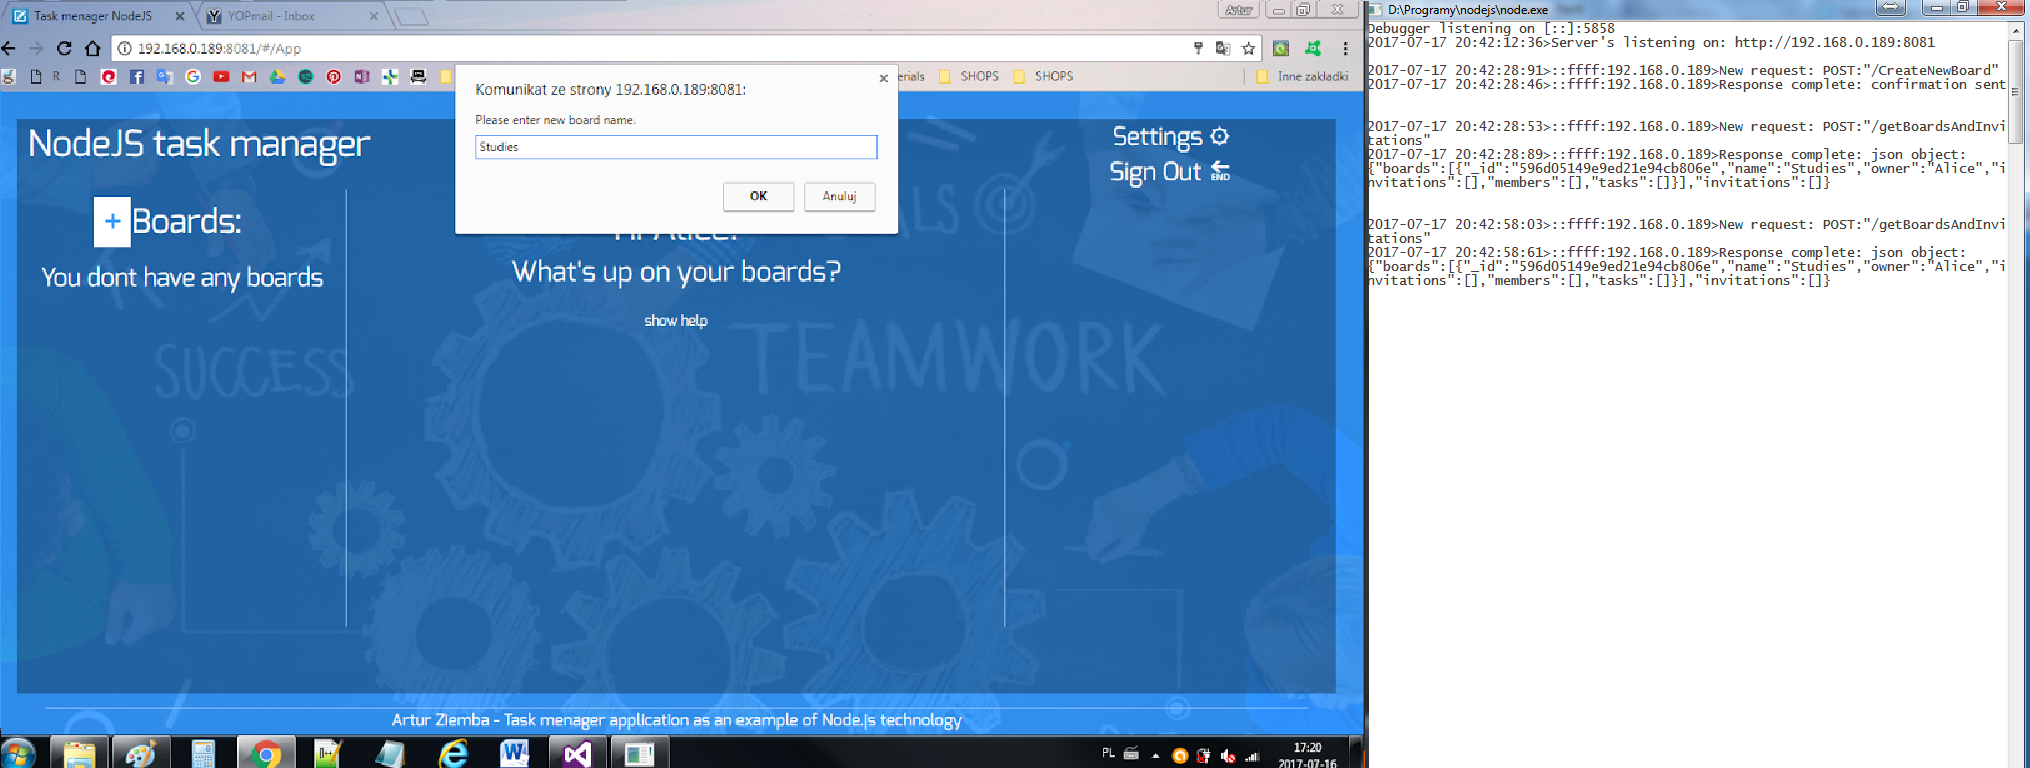
\includegraphics[width=\textwidth,height=\textheight,keepaspectratio]{72.png}
\captionsetup{labelformat=empty}
\caption[]{Po zalogowaniu się użytkownik wybiera opcje dodania tablicy, wpisuje wymagane dane i wysyła je do serwera. 
Serwer sprawdza poprawność danych. 
Jeśli są poprawne, serwer tworzy nową tablicę dla użytkownika i wysyła potwierdzenie w odpowiedzi.
W przeciwnym wypadku odpowiada komunikatem o błędzie.}
\end{figure}

\subsection{Wysyłanie zaproszenia do tablicy}
\begin{figure}[!hb]
\centering
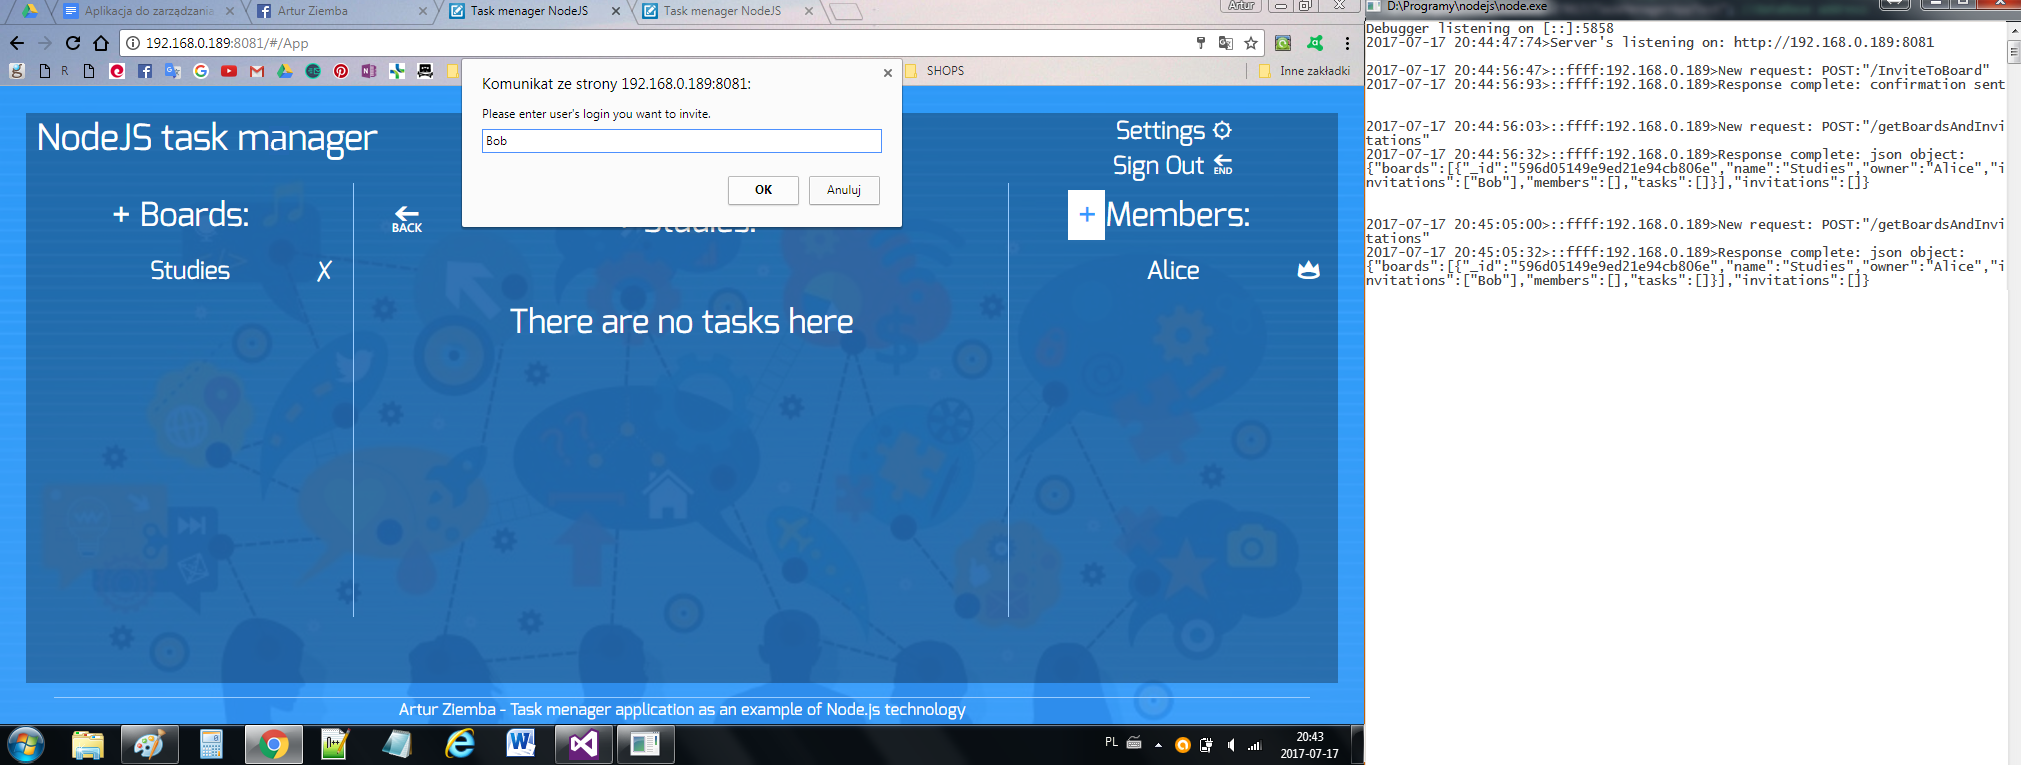
\includegraphics[width=\textwidth,height=\textheight,keepaspectratio]{02.png}
\captionsetup{labelformat=empty}
\caption[]{Po zalogowaniu się użytkownik wybiera opcje wysłania zaproszenia do wybranej tablicy, wypełnia dane i wysyła żądanie do serwera. Serwer sprawdza poprawność danych. 
W odpowiedzi wysyła potwierdzenie o wysłanym zaproszeniu lub komunikat o błędzie.}
\end{figure}

\newpage 
\subsection{Akceptacja zaproszenia}
\begin{figure}[!hb]
\centering
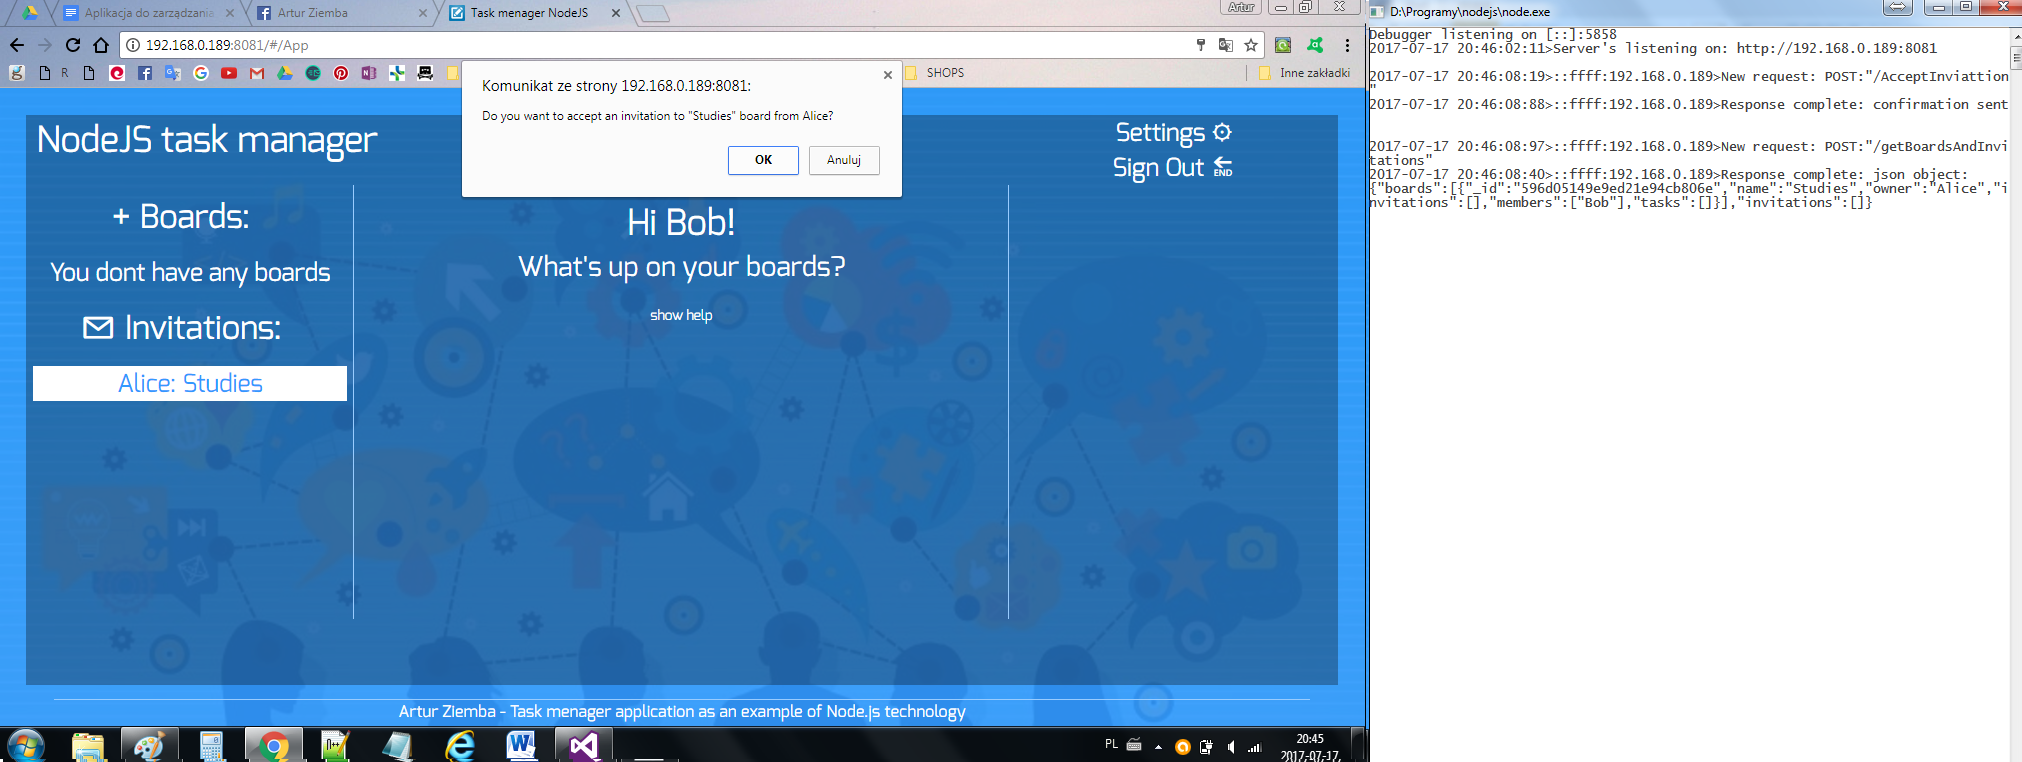
\includegraphics[width=\textwidth,height=\textheight,keepaspectratio]{82.png}
\captionsetup{labelformat=empty}
\caption[]{Po zalogowaniu się użytkownik wybiera opcje zaakceptowania oczekującego zaproszenia i wysyła żądanie do serwera. 
Serwer sprawdza poprawność danych. Odpowiada potwierdzeniem lub komunikatem o błędzie.}
\end{figure}

\subsection{Odrzucenie zaproszenia}
\begin{figure}[!hb]
\centering
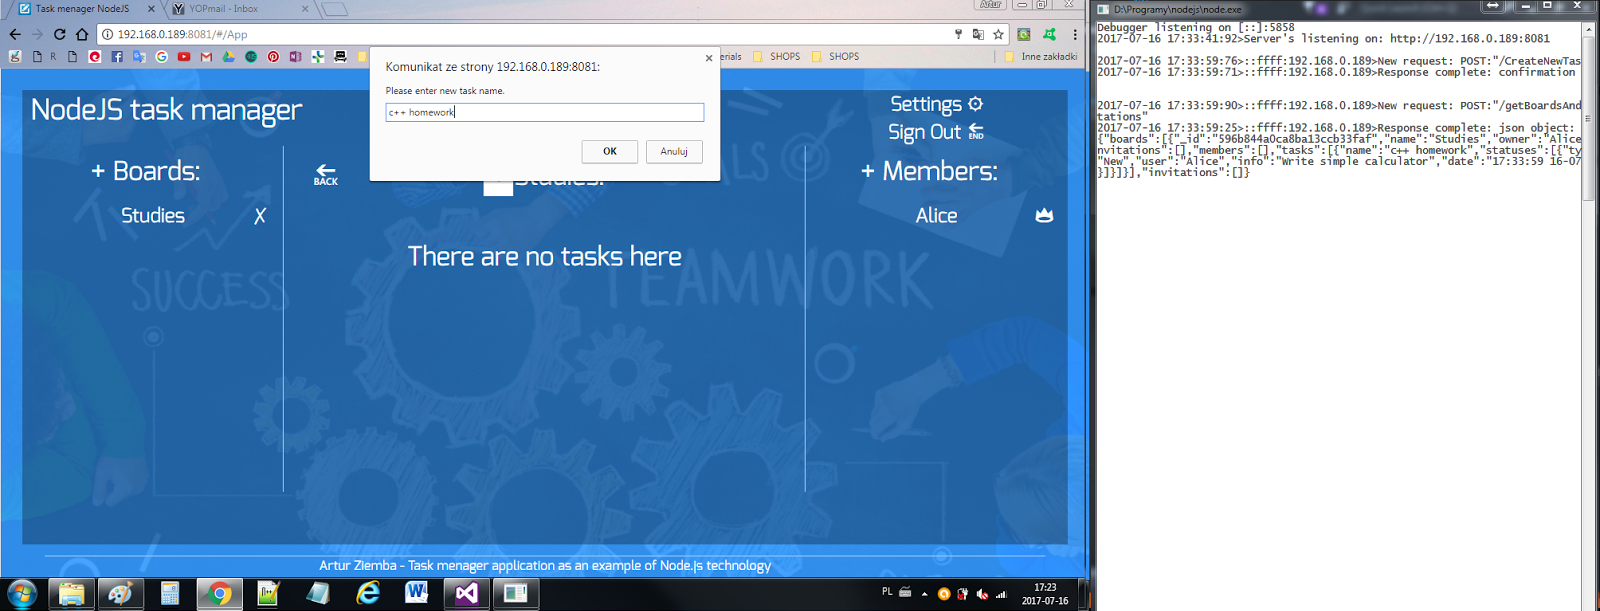
\includegraphics[width=\textwidth,height=\textheight,keepaspectratio]{A2.png}
\captionsetup{labelformat=empty}
\caption[]{Po zalogowaniu się użytkownik wybiera opcje odrzucenia oczekującego zaproszenia i wysyła żądanie do serwera. Serwer sprawdza poprawność danych. Odpowiada potwierdzeniem lub komunikatem o błędzie.}
\end{figure}

\newpage 
\subsection{Wyrzucenie użytkownika z tablicy}
\begin{figure}[!hb]
\centering
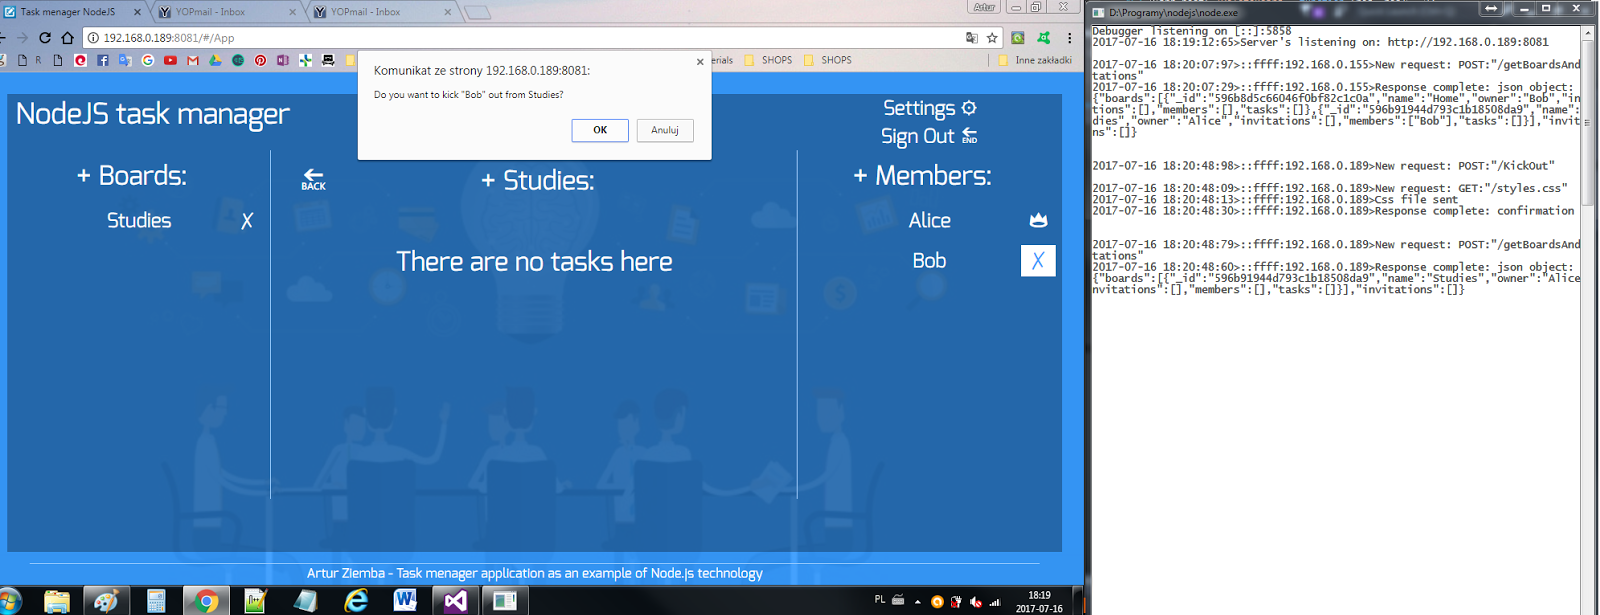
\includegraphics[width=\textwidth,height=\textheight,keepaspectratio]{92.png}
\captionsetup{labelformat=empty}
\caption[]{Po zalogowaniu się użytkownik wybiera opcje wyrzucenia użytkownika z określonej tablicy i wysyła żądanie do serwera. 
Serwer sprawdza poprawność danych. Odpowiada potwierdzeniem lub komunikatem o błędzie.}
\end{figure}

\subsection{Dodanie zadania}
\begin{figure}[!hb]
\centering
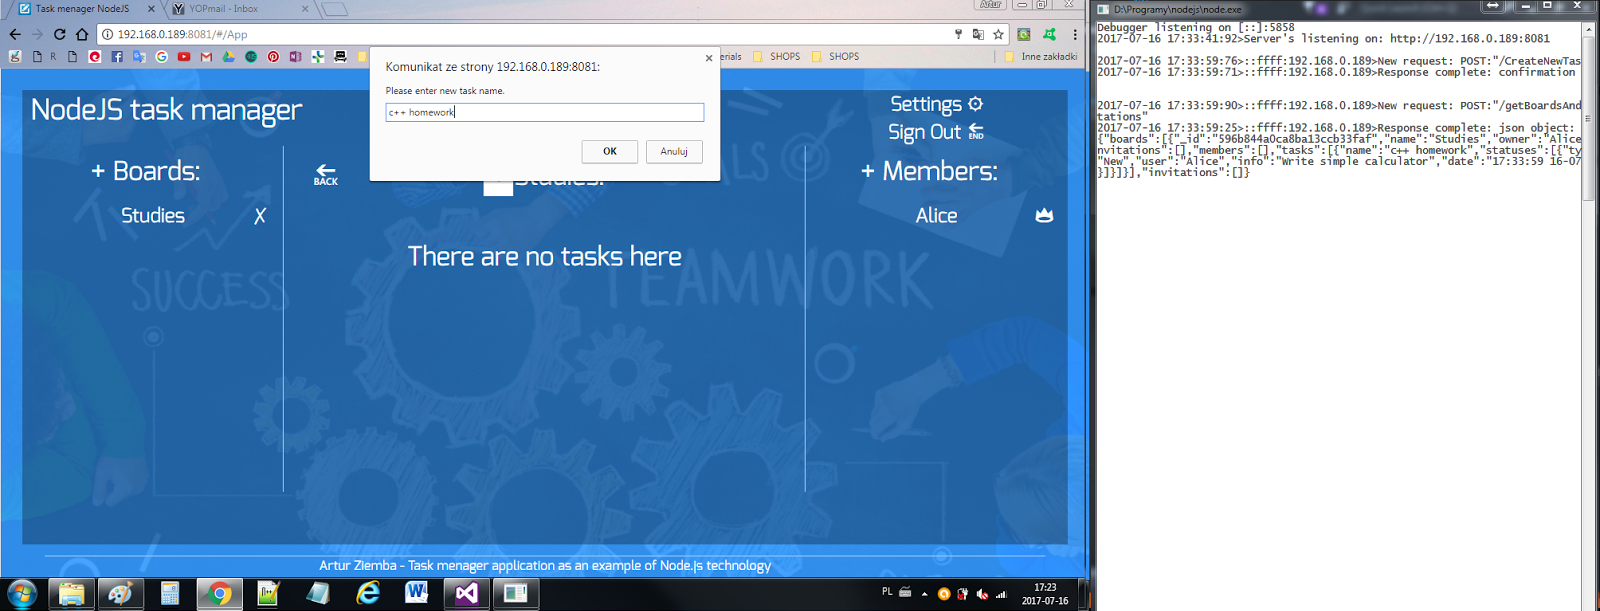
\includegraphics[width=\textwidth,height=\textheight,keepaspectratio]{A2.png}
\captionsetup{labelformat=empty}
\caption[]{Po zalogowaniu i wybraniu odpowiedniej tablicy użytkownik wybiera opcje dodania zadania, wypełnia dane i przesyła żądanie do serwera. 
Serwer sprawdza poprawność danych. Odpowiada potwierdzeniem lub komunikatem o błędzie.}
\end{figure}

\newpage 
\subsection{Dodanie statusu zadania}
\begin{figure}[!hb]
\centering
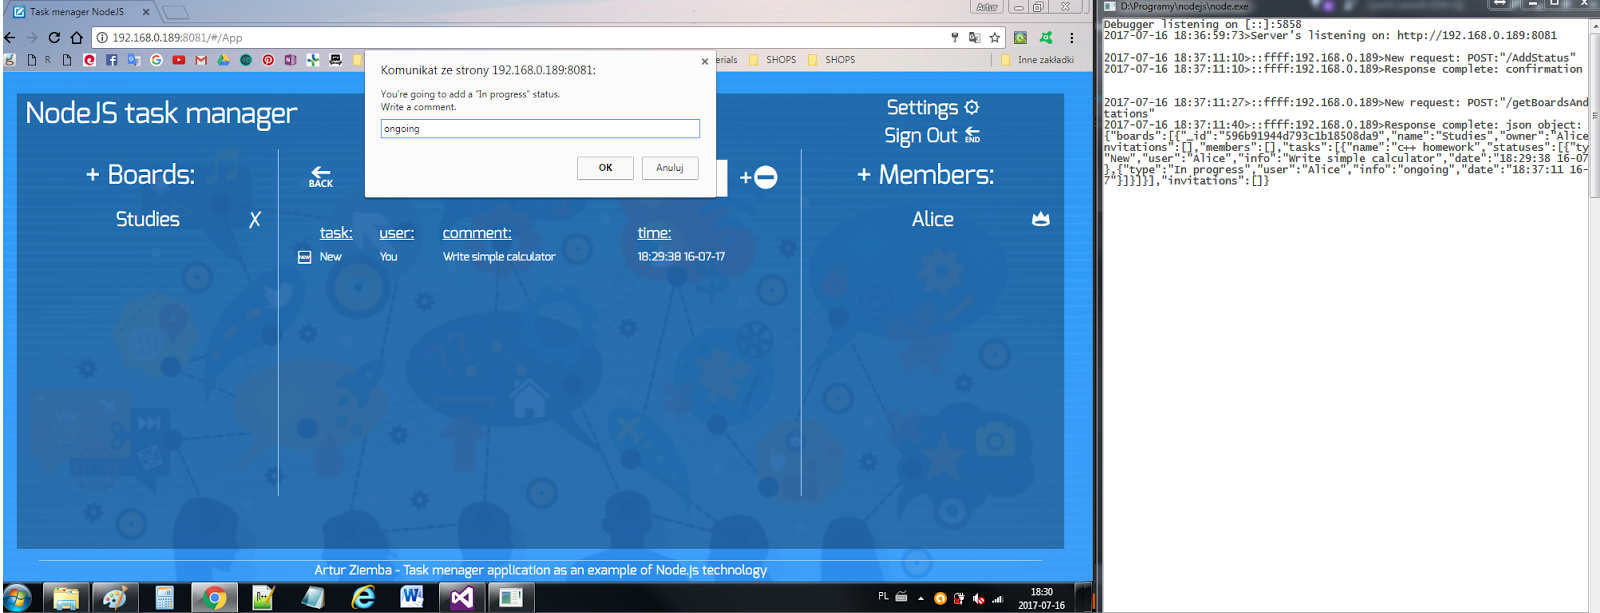
\includegraphics[width=\textwidth,height=\textheight,keepaspectratio]{B2.png}
\captionsetup{labelformat=empty}
\caption[]{Po zalogowaniu, wybraniu odpowiedniej tablicy i zadania użytkownik wybiera opcje dodania nowego statusu, uzupełnia dane i przesyła żądanie do serwera. 
Serwer sprawdza poprawność danych. Odpowiada potwierdzeniem lub komunikatem o błędzie.}
\end{figure}

\subsection{Usuwanie zadania}
\begin{figure}[!hb]
\centering
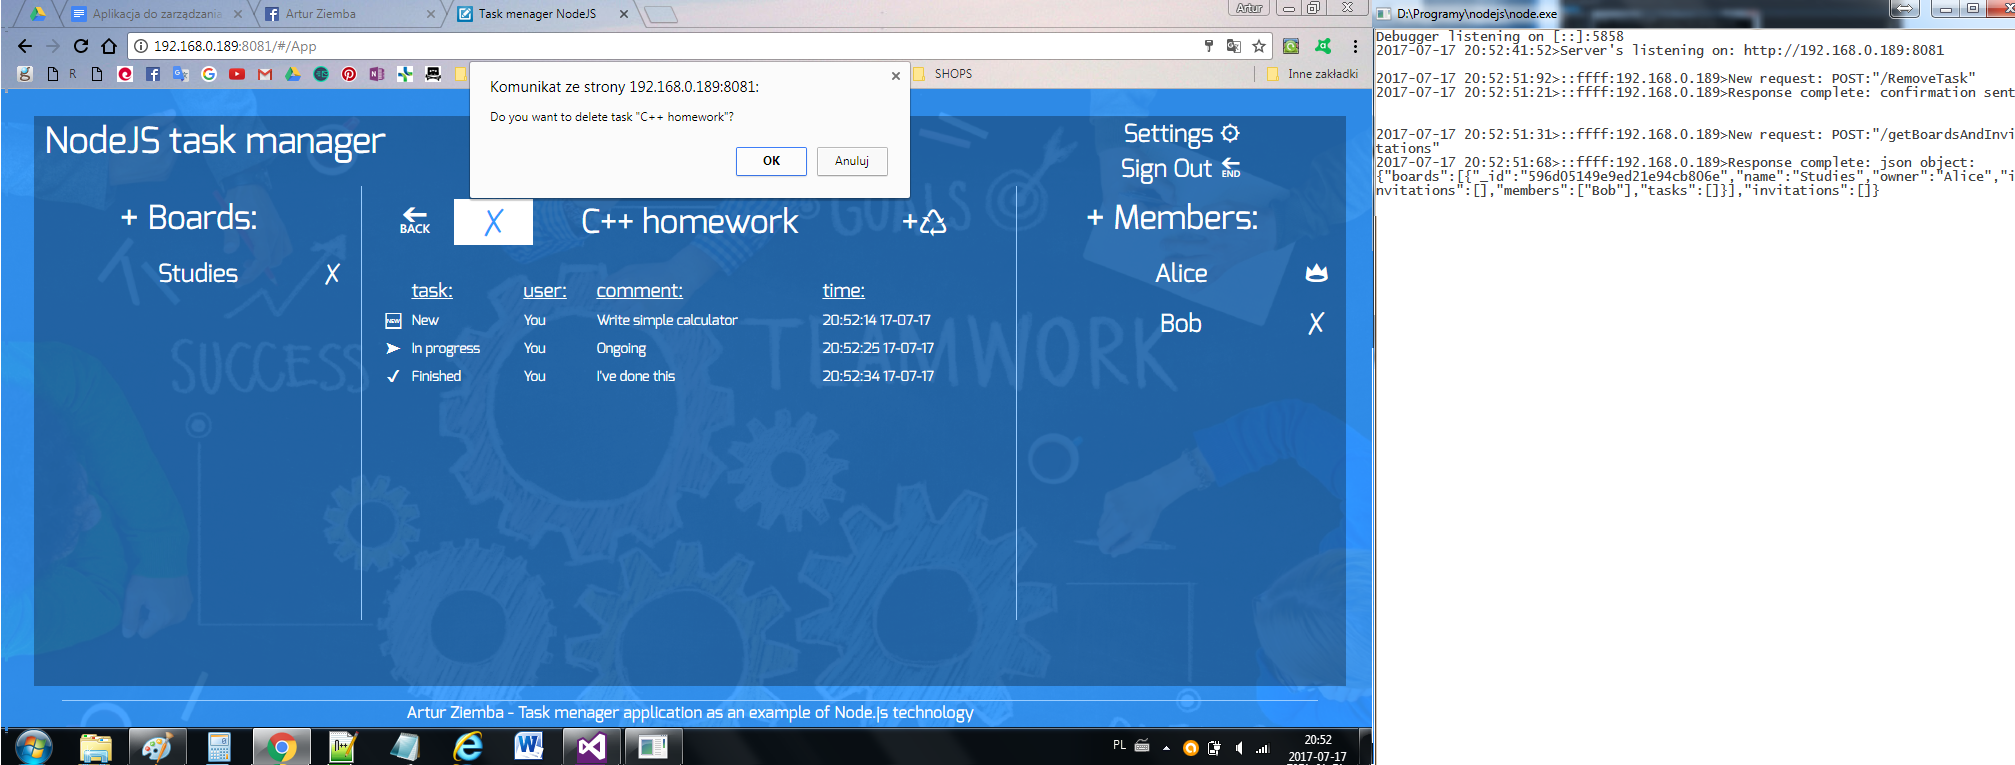
\includegraphics[width=\textwidth,height=\textheight,keepaspectratio]{C2.png}
\captionsetup{labelformat=empty}
\caption[]{Po zalogowaniu, wybraniu odpowiedniej tablicy i zakończonego zadania użytkownik wybiera opcje usuwania zadania i przesyła żądanie do serwera. 
Serwer sprawdza poprawność danych. Odpowiada potwierdzeniem lub komunikatem o błędzie.}
\end{figure}

\newpage 
\subsection{Opuszczanie tablicy}
\begin{figure}[!hb]
\centering
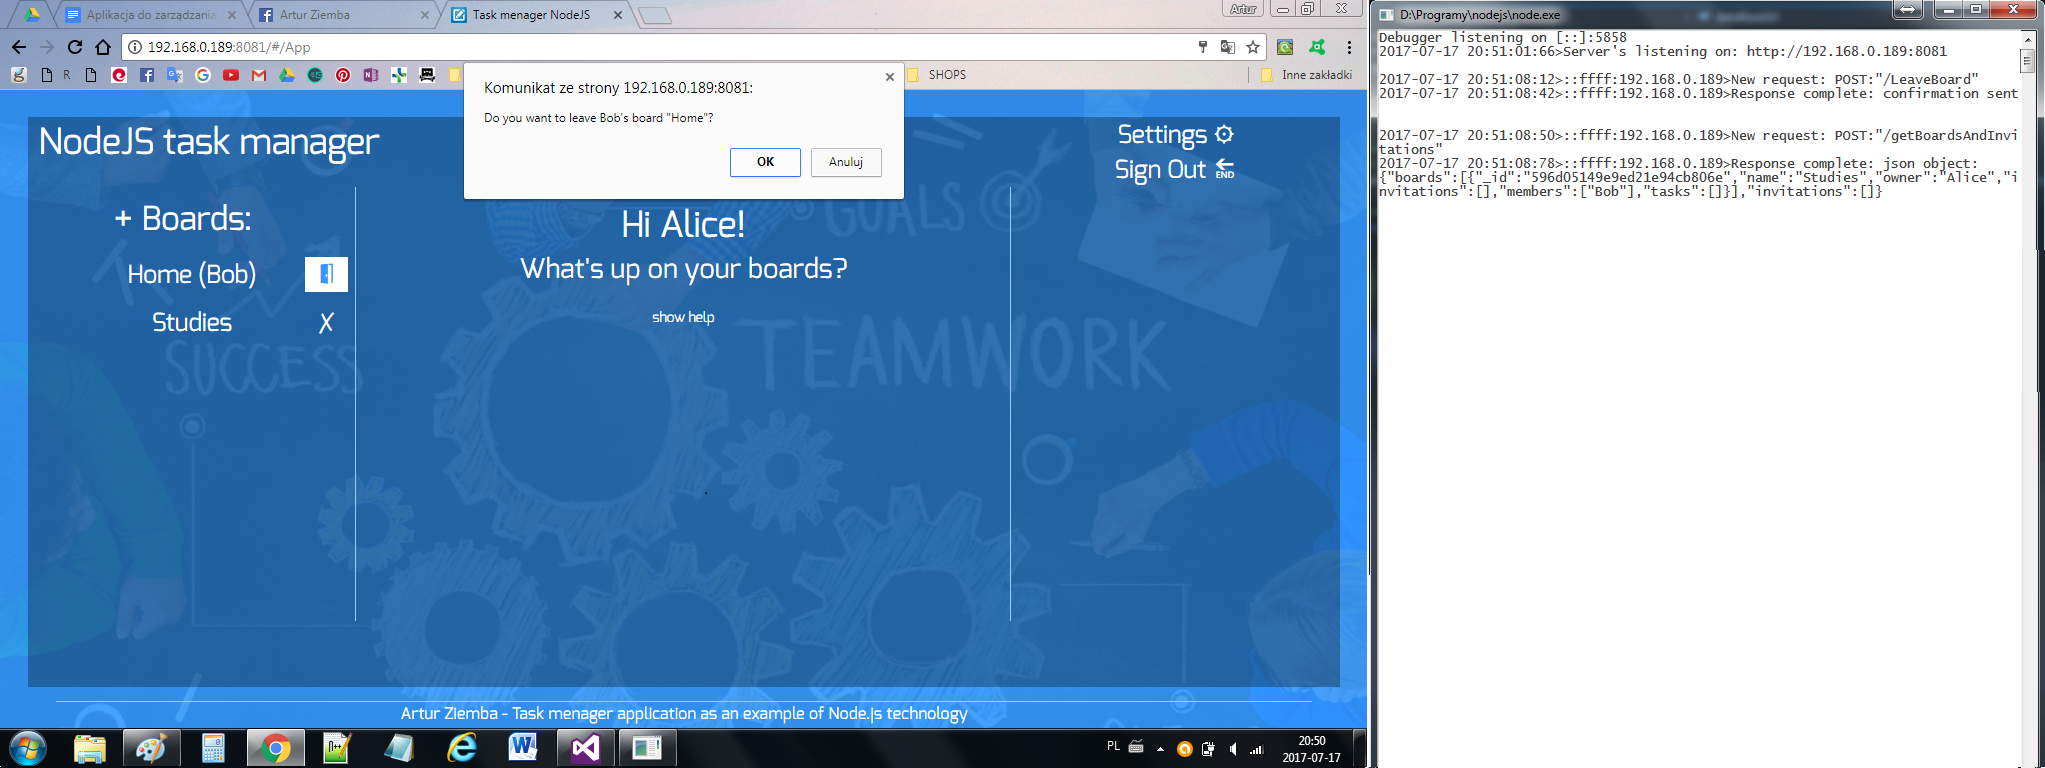
\includegraphics[width=\textwidth,height=\textheight,keepaspectratio]{D2.png}
\captionsetup{labelformat=empty}
\caption[]{Po zalogowaniu użytkownik wybiera opcje opuszczenia tablicy, której jest członkiem i wysyła żądanie do serwera. 
Serwer sprawdza poprawność danych. Odpowiada potwierdzeniem lub komunikatem o błędzie.}
\end{figure}

\subsection{Usuwanie tablicy}
\begin{figure}[!hb]
\centering
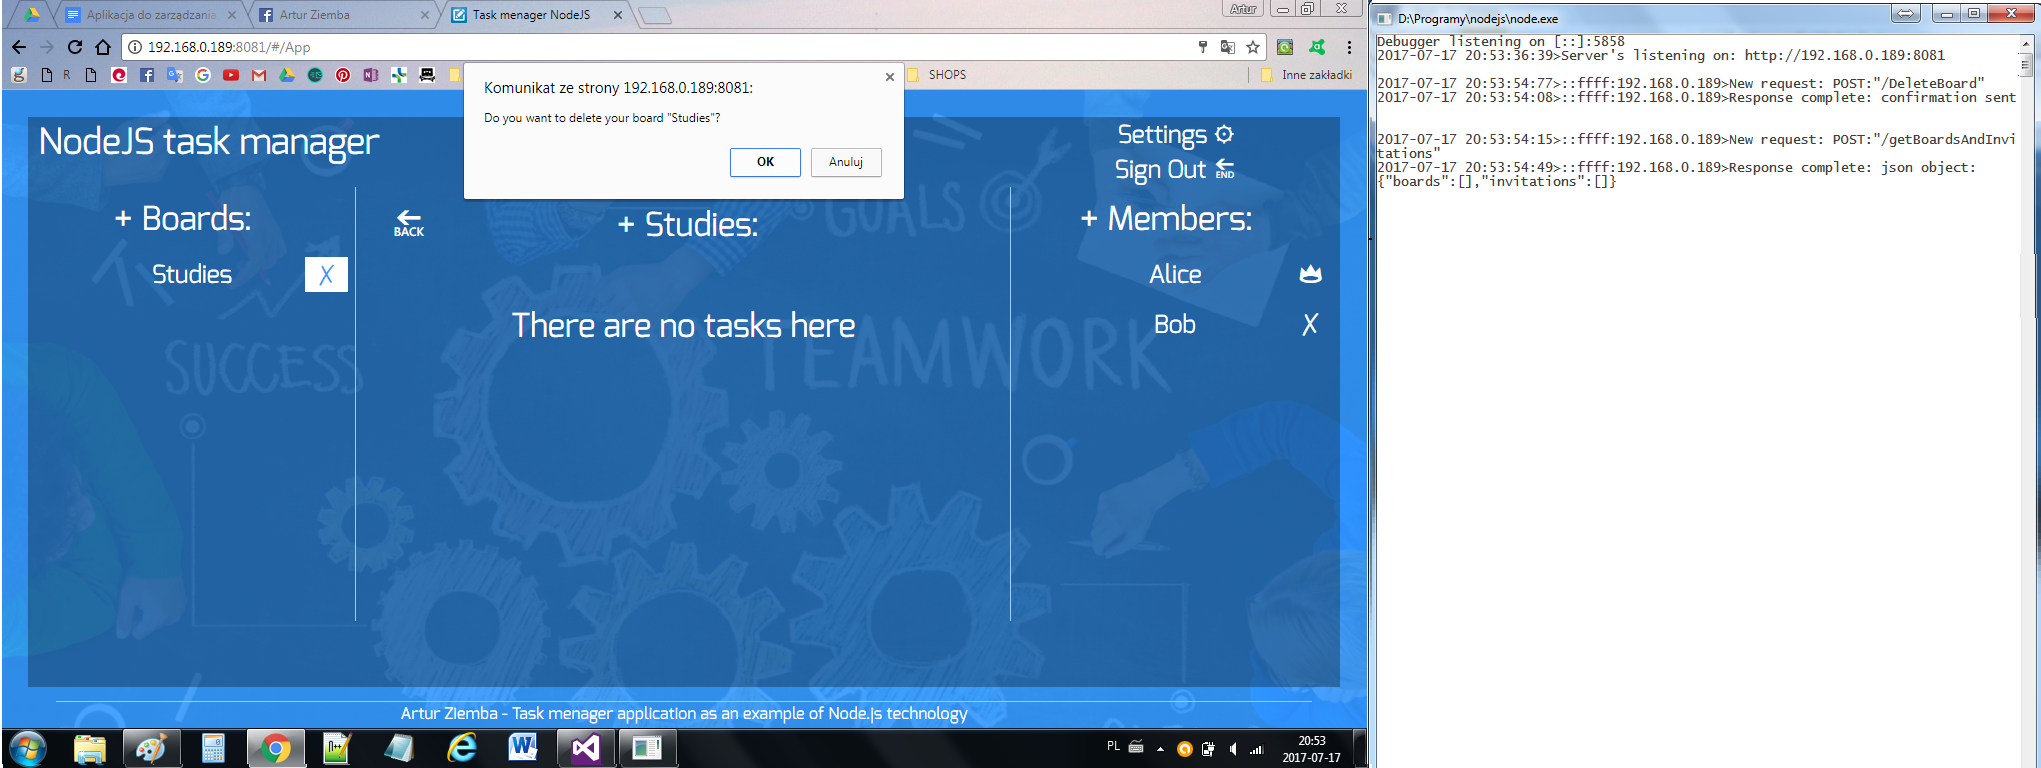
\includegraphics[width=\textwidth,height=\textheight,keepaspectratio]{E2.png}
\captionsetup{labelformat=empty}
\caption[]{Po zalogowaniu użytkownik wybiera opcje usunięcia własnej tablicy i wysyła żądanie do serwera. Serwer sprawdza poprawność danych. Odpowiada potwierdzeniem lub komunikatem o błędzie.}
\end{figure}

\section{Testy wydajnościowe}
Przeprowadzone testy wydajnościowe pozwalają sprawdzić zachowanie serwisu przy różnym obciążeniu bazy danych. Każdy test został wykonany 5 razy, a podane wartości przedstawiają średnią czasu pracy.

\begin{enumerate} 
	\item
	Mała ilość danych - 5 użytkowników po 2 tablice, po 3 zadania, po 2 komentarze
	\begin{itemize}
	  \item logowanie - 22ms
	  \item otrzymanie informacji o tablicach i zaproszeniach - 29ms
	  \item dodanie nowej tablicy - 20ms
	  \item dodanie nowego zadania - 27ms
	  \item dodanie komentarza - 26ms
	\end{itemize}
	\item
	Średnia ilość danych - 50 użytkowników po 4 tablice, po 6 zadań, po 5 komentarzy
	\begin{itemize}
	  \item logowanie - 26ms
	  \item otrzymanie informacji o tablicach i zaproszeniach - 33ms
	  \item dodanie nowej tablicy - 27ms
	  \item dodanie nowego zadania - 35ms
	  \item dodanie komentarza - 30ms
	\end{itemize}
	\item
	Duża ilość danych - 500 użytkowników po 8 tablic, po 12 zadań, po 11 komentarzy
	\begin{itemize}
	  \item logowanie - 32ms
	  \item otrzymanie informacji o tablicach i zaproszeniach - 39ms
	  \item dodanie nowej tablicy - 31ms
	  \item dodanie nowego zadania - 37ms
	  \item dodanie komentarza - 32ms
	\end{itemize}
\end{enumerate} 
Serwis oferuje pełną funkcjonalność przy różnych obciążeniach bazy danych. Mimo dużej ilości posiadanych informacji korzystanie z serwisu jest komfortowe, ponieważ czas obsługi zapytania nie zostaje znacząco wydłużony.

\section{Testy obciążeniowe serwera}
Przeprowadzone testy pozwalają określić zachowanie aplikacji w przypadku równoczesnej obsługi wielu przychodzących zapytań. Każdy test został wykonany 5 razy, a podane wartości przedstawiają średnią czasu pracy.
\smallskip
\begin{center}
  \begin{tabular}{ | c | c | }
    \hline
    & czas otrzymania odpowiedzi \\
    \hline
	Mała ilość danych - 50 jednocześnie wysłanych zapytań & 45ms \\
	\hline
	Średnia ilość danych - 300 jednocześnie wysłanych zapytań & 121ms \\
	\hline
	Duża ilość danych - 1500 jednocześnie wysłanych zapytań & 674ms \\
    \hline
  \end{tabular}
\end{center}
\bigskip\medskip

Serwis oferuje pełną funkcjonalność przy różnym stopniu obciążenia serwera. Przy dużej liczbie przychodzących zapytań użytkowanie serwisu jest wciąż komfortowe. Aplikacja wykazuje się skalowalnością.

\section{Testy sprawnościowe serwera}
Przeprowadzone testy pozwalają określić ilość kolejno wysłanych po sobie zapytań, które zostały obsłużone przez serwer w określonym czasie. Każdy test został wykonany 5 razy, a podane wartości przedstawiają średnią czasu pracy.
\bigskip \medskip
\begin{center}
  \begin{tabular}{ | c | c | }
    \hline
    & ilość otrzymanych odpowiedzi\\
    \hline
	Mały okres czasu - 1 sekunda & 139 \\
	\hline
	Średni okres czasu - 30 sekund & 4723 \\
	\hline
	Duży okres czasu - 5 minut & 48031 \\
    \hline
  \end{tabular}
\end{center}
\bigskip \medskip
Przedstawione wyniki prezentują możliwości obsługi kolejnych zapytań serwera Node.js. 
Osiągnięte wyniki są zadowalające, jednak łatwo zauważyć, że technologia ta wykazuje się największą sprawnością przy obsłudze równoległych zapytań. 
Średni uzyskany czas dla obsługi 1500 zapytań równoległych to 674 ms, natomiast dla wysyłanych kolejno wynosi 940 ms.


\chapter{Podsumowanie otrzymanych wyników i wnioski na temat środowiska}
Wykonana aplikacja spełnia zadaną w warunkach funkcjonalność. 
Zostały osiągnięte wszystkie założenia oraz wymagania aplikacji przy użyciu możliwości dostarczanej przez technologię Node.js. 
Stworzony projekt doskonale nadaje się do użytkowania przez zorganizowane zespoły do wykonywania określonych zadań. 
Mógłby być na przykład używany do zarządzania pracą zespołów deweloperskich pracujących w różnych metodykach takich jak scrum czy kanban. 
Dostarcza przejrzysty interfejs oraz nieskomplikowaną prezentację danych dla końcowych użytkowników, przez co nie wymaga praktycznie żadnych szkoleń lub procesów wdrożeniowych w celu zdobycia umiejętności biegłej obsługi narzędzia. 
Środowisko Node.js wydaje się być bardzo nowoczesnym oraz przyszłościowym środowiskiem. 
Niewątpliwie największymi zaletami tej technologii jest łatwość budowania wymagających serwisów internetowych poprzez użycie asynchronicznej obsługi wejścia/wyjścia, które pozwala na przetwarzanie wielu funkcji w jednym czasie, tworząc wyjątkowo szybkie w działaniu aplikacje. 
Zagadnienie to wymaga jednak umiejętności w projektowaniu i analizowaniu funkcji programowania asynchronicznego. 
Kod pisany jest w szeroko używanym języku JavaScript, co zbudowało ogromną społeczność zainteresowaną technologią Node.js. 
Dzięki temu możemy z łatwością zdobyć materiały przydatne w procesie poznawczym środowiska. 
Globalne repozytorium npm gwarantuje obsługę wielu funkcjonalności, bez potrzeby długiego szukania możliwych rozwiązań. 
Wszystko jest dostępne bezpłatnie, gotowe do wdrożenia w tworzonej aplikacji. 
Mimo, że jest to technologia stosunkowo młoda, obecnie Node.js jest używany, a co za tym idzie, sprawdzony przez największe firmy IT w celu obsługi ich aplikacji i serwerów. 
Należy być świadomym wszystkich zalet i wad przy wyborze określonej technologii. 
Node.js nie nadaje się do każdego typu projektu. 
Nie jest efektywnym środowiskiem w korzystaniu z obliczeń intensywnie wykorzystujących procesor. 
Jest on natomiast idealnym rozwiązaniem w kwestii pracy nad wieloma rozwiązaniami webowymi. 
Osobiście praca w Node.js sprawiła mi wielką radość i stała się moją ulubioną technologią dzięki zapewnionej prostocie i możliwych do uzyskania bez większego wysiłku ogromnych możliwościach.

\addcontentsline{toc}{chapter}{Bibliografia} 
\begin{thebibliography}{99}
\bibitem{Brown}
E. Brown
\textit{"Web Development with Node and Express", 2014}
\bibitem{Onodi}
R. Onodi
\textit{"MEAN Blueprints", 2016}
\bibitem{AngulrJS}
P. Kozlowski, P. B. Darwin
\textit{"Mastering Web Application Development with AngularJS", 2013}
\bibitem{node eff}
D. Resende 
\textit{"Node.js High Performance", 2015}
\bibitem{js eff}
N. Zakas
\textit{"High Performance JavaScript", 2010}
\bibitem{libuv}
N. Marathe
\textit{"An Introduction to libuv", 2012}
\bibitem{Node vs Ringojs}
H. Wallnöfer
\textit{porównanie technologii Node.js i Ringojs, 2010, źródło: http://hns.github.io/2010/09/21/benchmark.html}
\bibitem{Node.js}
Node.js Foundation
\textit{dokumentacja języka programowania Node.js, 2017, źródło: https://nodejs.org/en/docs/}
\bibitem{MongoDB}
MongoDB, Inc.
\textit{dokumentacja MongoDB, 2017, źródło: https://docs.mongodb.com/}
\bibitem{Ringojs}
Ringojs
\textit{dokumentacja Ringojs, 2017, źródło: https://ringojs.org/}
\bibitem{Twisted}
Wikipedia
\textit{artykuł poświęcony technolgii Twisted, 2017, źródło: https://en.wikipedia.org/wiki/Twisted\_(software)}
\bibitem{Node.js wiki}
Wikipedia
\textit{artykuł poświęcony technolgii Node.js, 2017, źródło: https://en.wikipedia.org/wiki/Node.js}
\bibitem{Vert.x}
Wikipedia
\textit{artykuł poświęcony technolgii Vert.x, 2017, źródło: https://en.wikipedia.org/wiki/Vert.x}
\end{thebibliography}
\addcontentsline{toc}{chapter}{Spis rysunków} 
\listoffigures

\end{document}